\chapter{Instrumentation}
\label{chp:instrumentation}
The author is leading the Group for the Advancement in Automation and Instrumentation (GAIA).
GAIA is the group responsible for maintaining, servicing, and upgrading hardware and software related to the observatory.

\section{Dome}
Dr.\ Cristina Valeria Torres Memorial Astronomical Observatory (CTMO) inaugurated May 5, 2018. 
Formerly Nompuewenu Observatory.
The word Nompuewenu meaning ``beyond the sky'' is borrowed from the Mapuche language used by the Mapuche people indigenous to Argentina.

\begin{figure}[h]
    \centering
    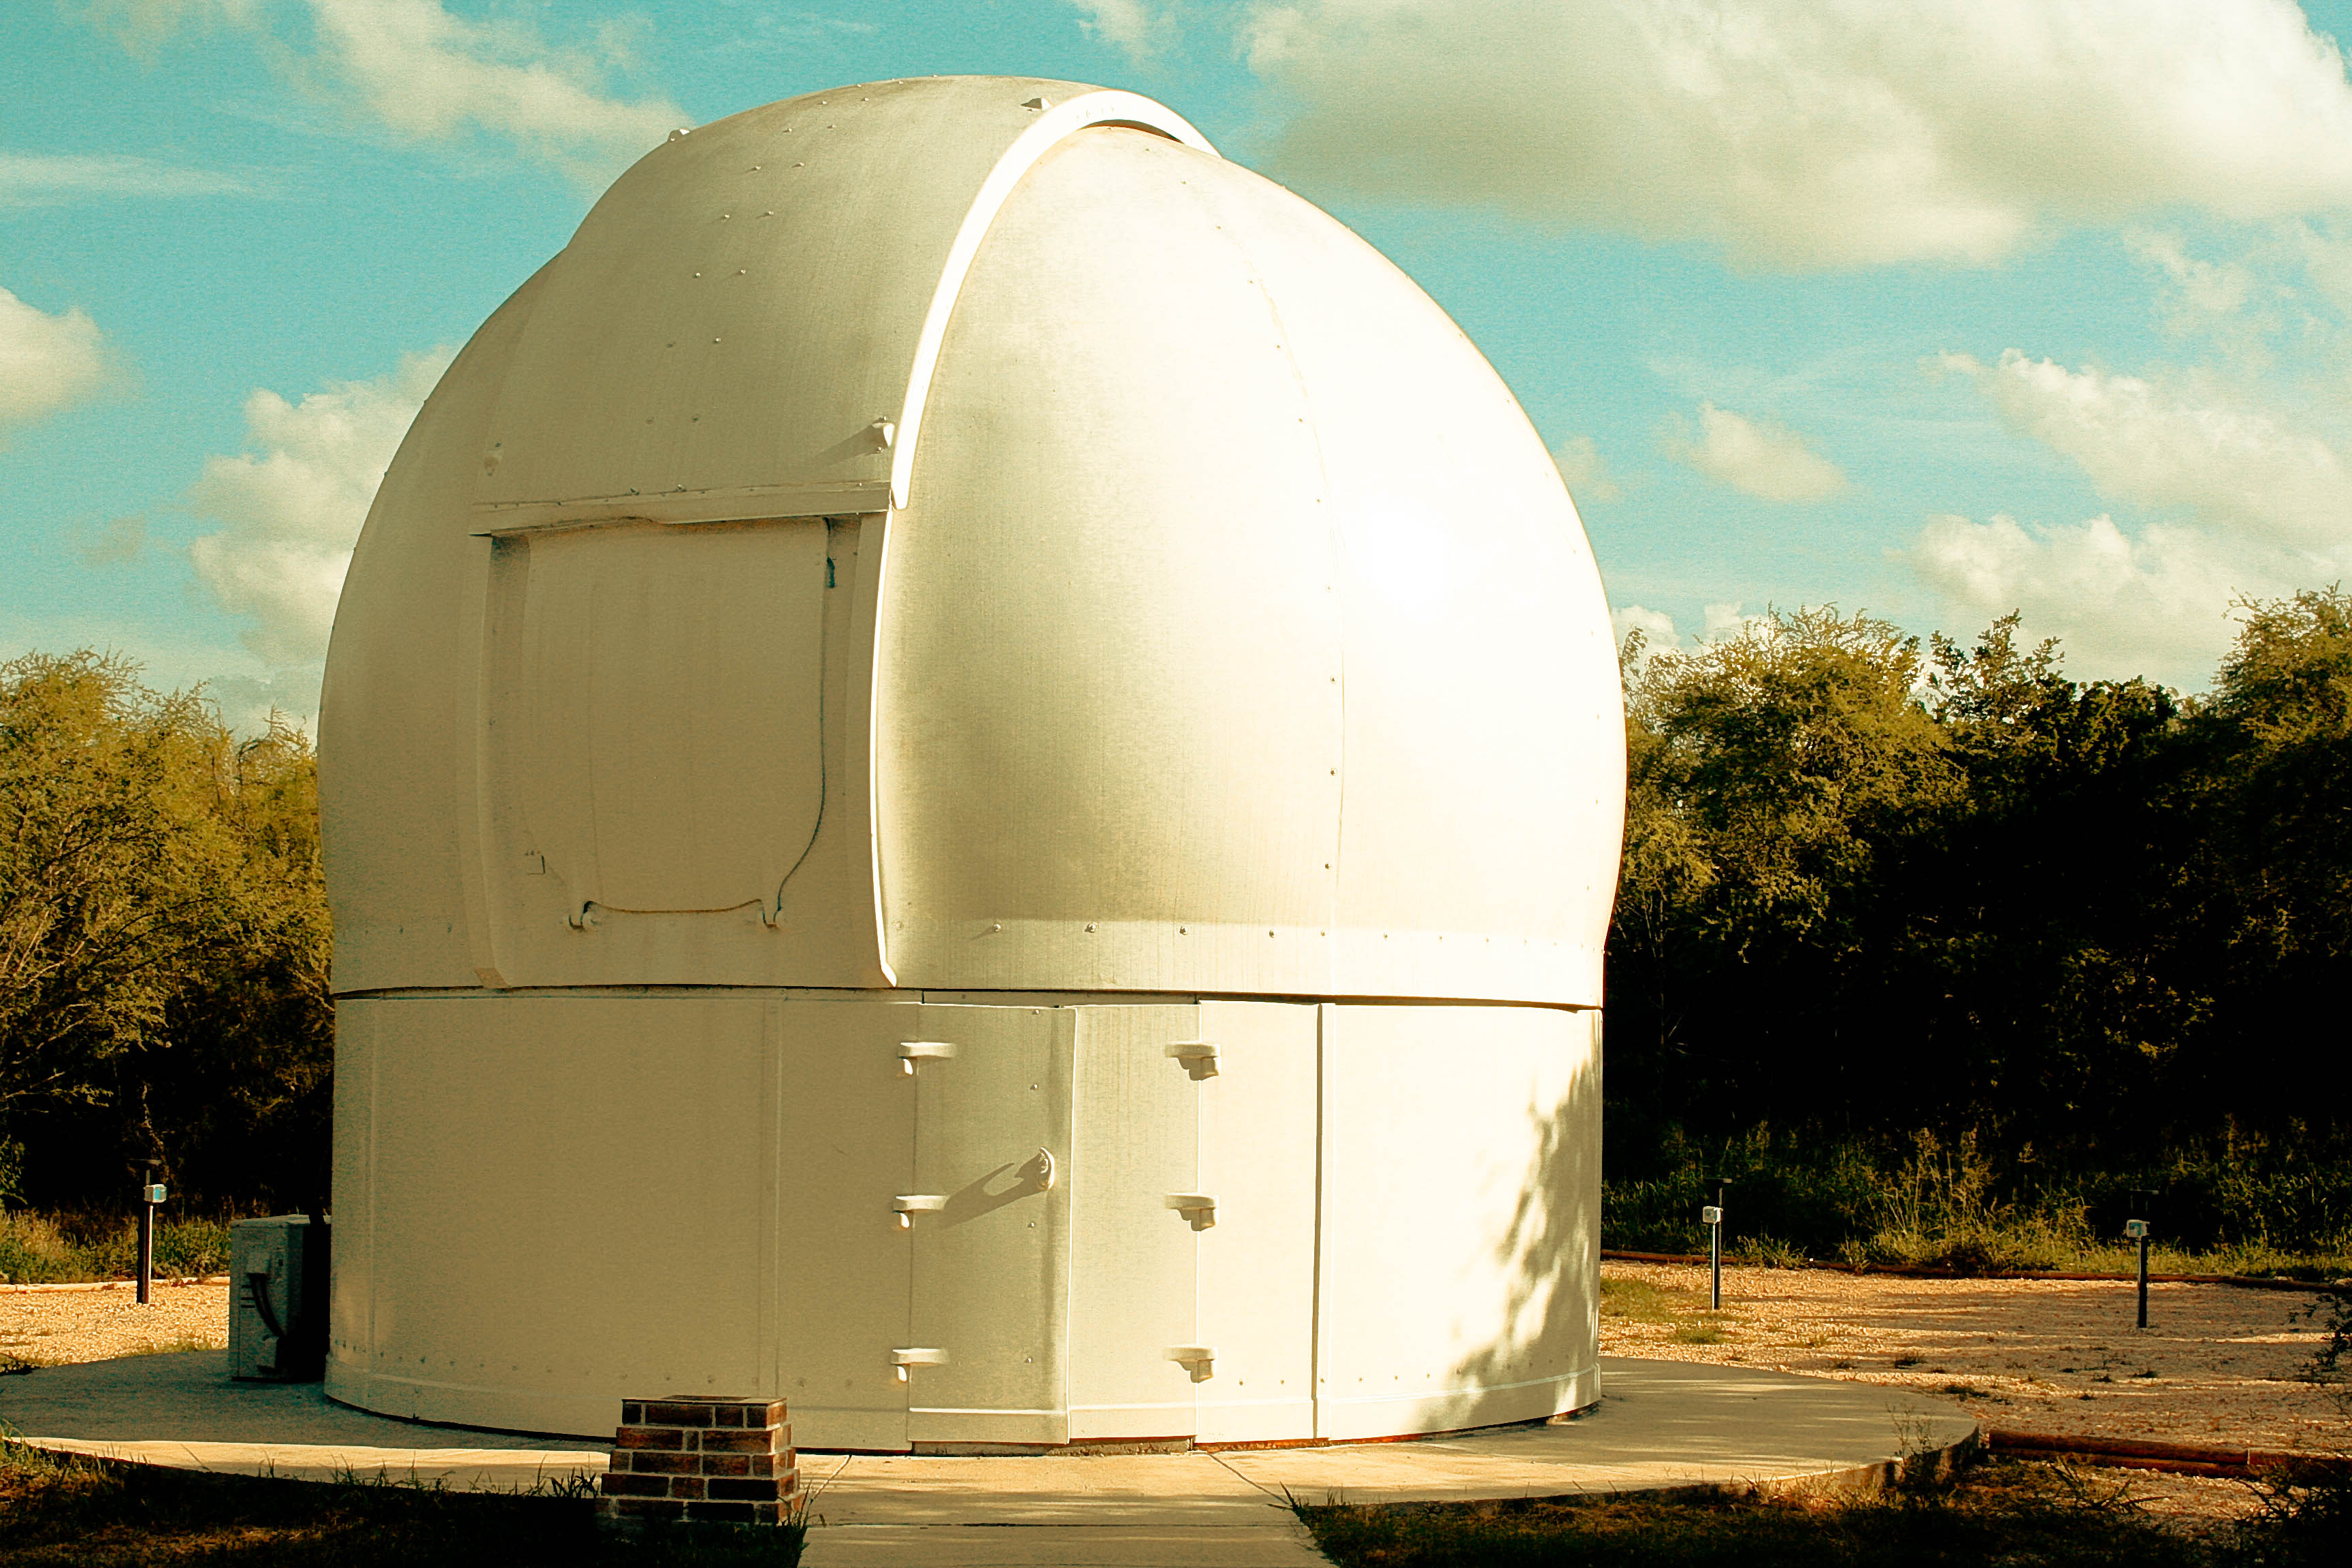
\includegraphics[width=\columnwidth]{figures/ctmo.jpg}%{example-image}
\caption{Dr.\ Cristina Valeria Torres Memorial Astronomical Observatory at Resaca de la Palma State Park photo by Americo Hinojosa Lee}
\label{fig:CTMO}
\end{figure}

The observatory was first constructed on the Brownsville campus of UTRGV\@.
With a growing downtown and campus light pollution became a serious issue for the observatory.
Alumn Antonio Galan scouted the region for a suitable location to relocate.
Former State Park Superintendent Pablo Deyturbe found Galan scouting the area near Resaca de la Palma State Park (RDLP).
Director of the Center for Gravitational Wave Astronomy (CGWA) Mario Diaz and Deyturbe worked together to establish  
a Memorandum of Understanding between UTRGV and Texas Parks and Wildlife Department (TPWD) to allow the relocation
of the observatory to be Resaca de la Palma State Park.

The dome is a custom build with all parts manufactured uniquely for this research and educational facility.

\subsection{Specifications}
\begin{description}
    \item[Observatory style] Dome shape
    \item[Window] Two parts, upper slides along domed roof; bottom opens draw bridge style
    \item[Wall height] 88 inches
    \item[Average Diameter] 245 inches\footnote{Average diameter is used since all domes increase in eccentricity or become egg shaped over time}
    \item[Approximate Height] 25 feet
\end{description}

\subsection{Robotizing of dome for remote operation}
The author is leading efforts to robotize the observatory and instrumentation for remote and autonomous operation.
The motors that control the shutter door and rotation are controlled manually.
For optimal control of the observatory, robotizing these controls is required.
These are the planned upgrades for the observatory.
\begin{itemize}
    \item Add hydraulic lift system to control shutter draw bridge door
    \item Implement wireless communication for shutter window and door control
    \item Add gear encoding to dome rotation motor using a rotary sensor
    \item Add cardinal position encoding using permanent magnets and hall effect sensors
    \item Use scripts to create nightly observation queues based on requests and LIGO\footnote{Laser Interferometer Gravitational Wave Observatory} alerts for Optical Followups of Gravitational Wave Events
    \item Develop drivers for communicating with sensors and observatory software
\end{itemize}

\subsection{Hardware}
The author has created prototypes of sensors to use for gear encoding with optical and hall effect sensors.

\begin{figure}[h]
    \centering
    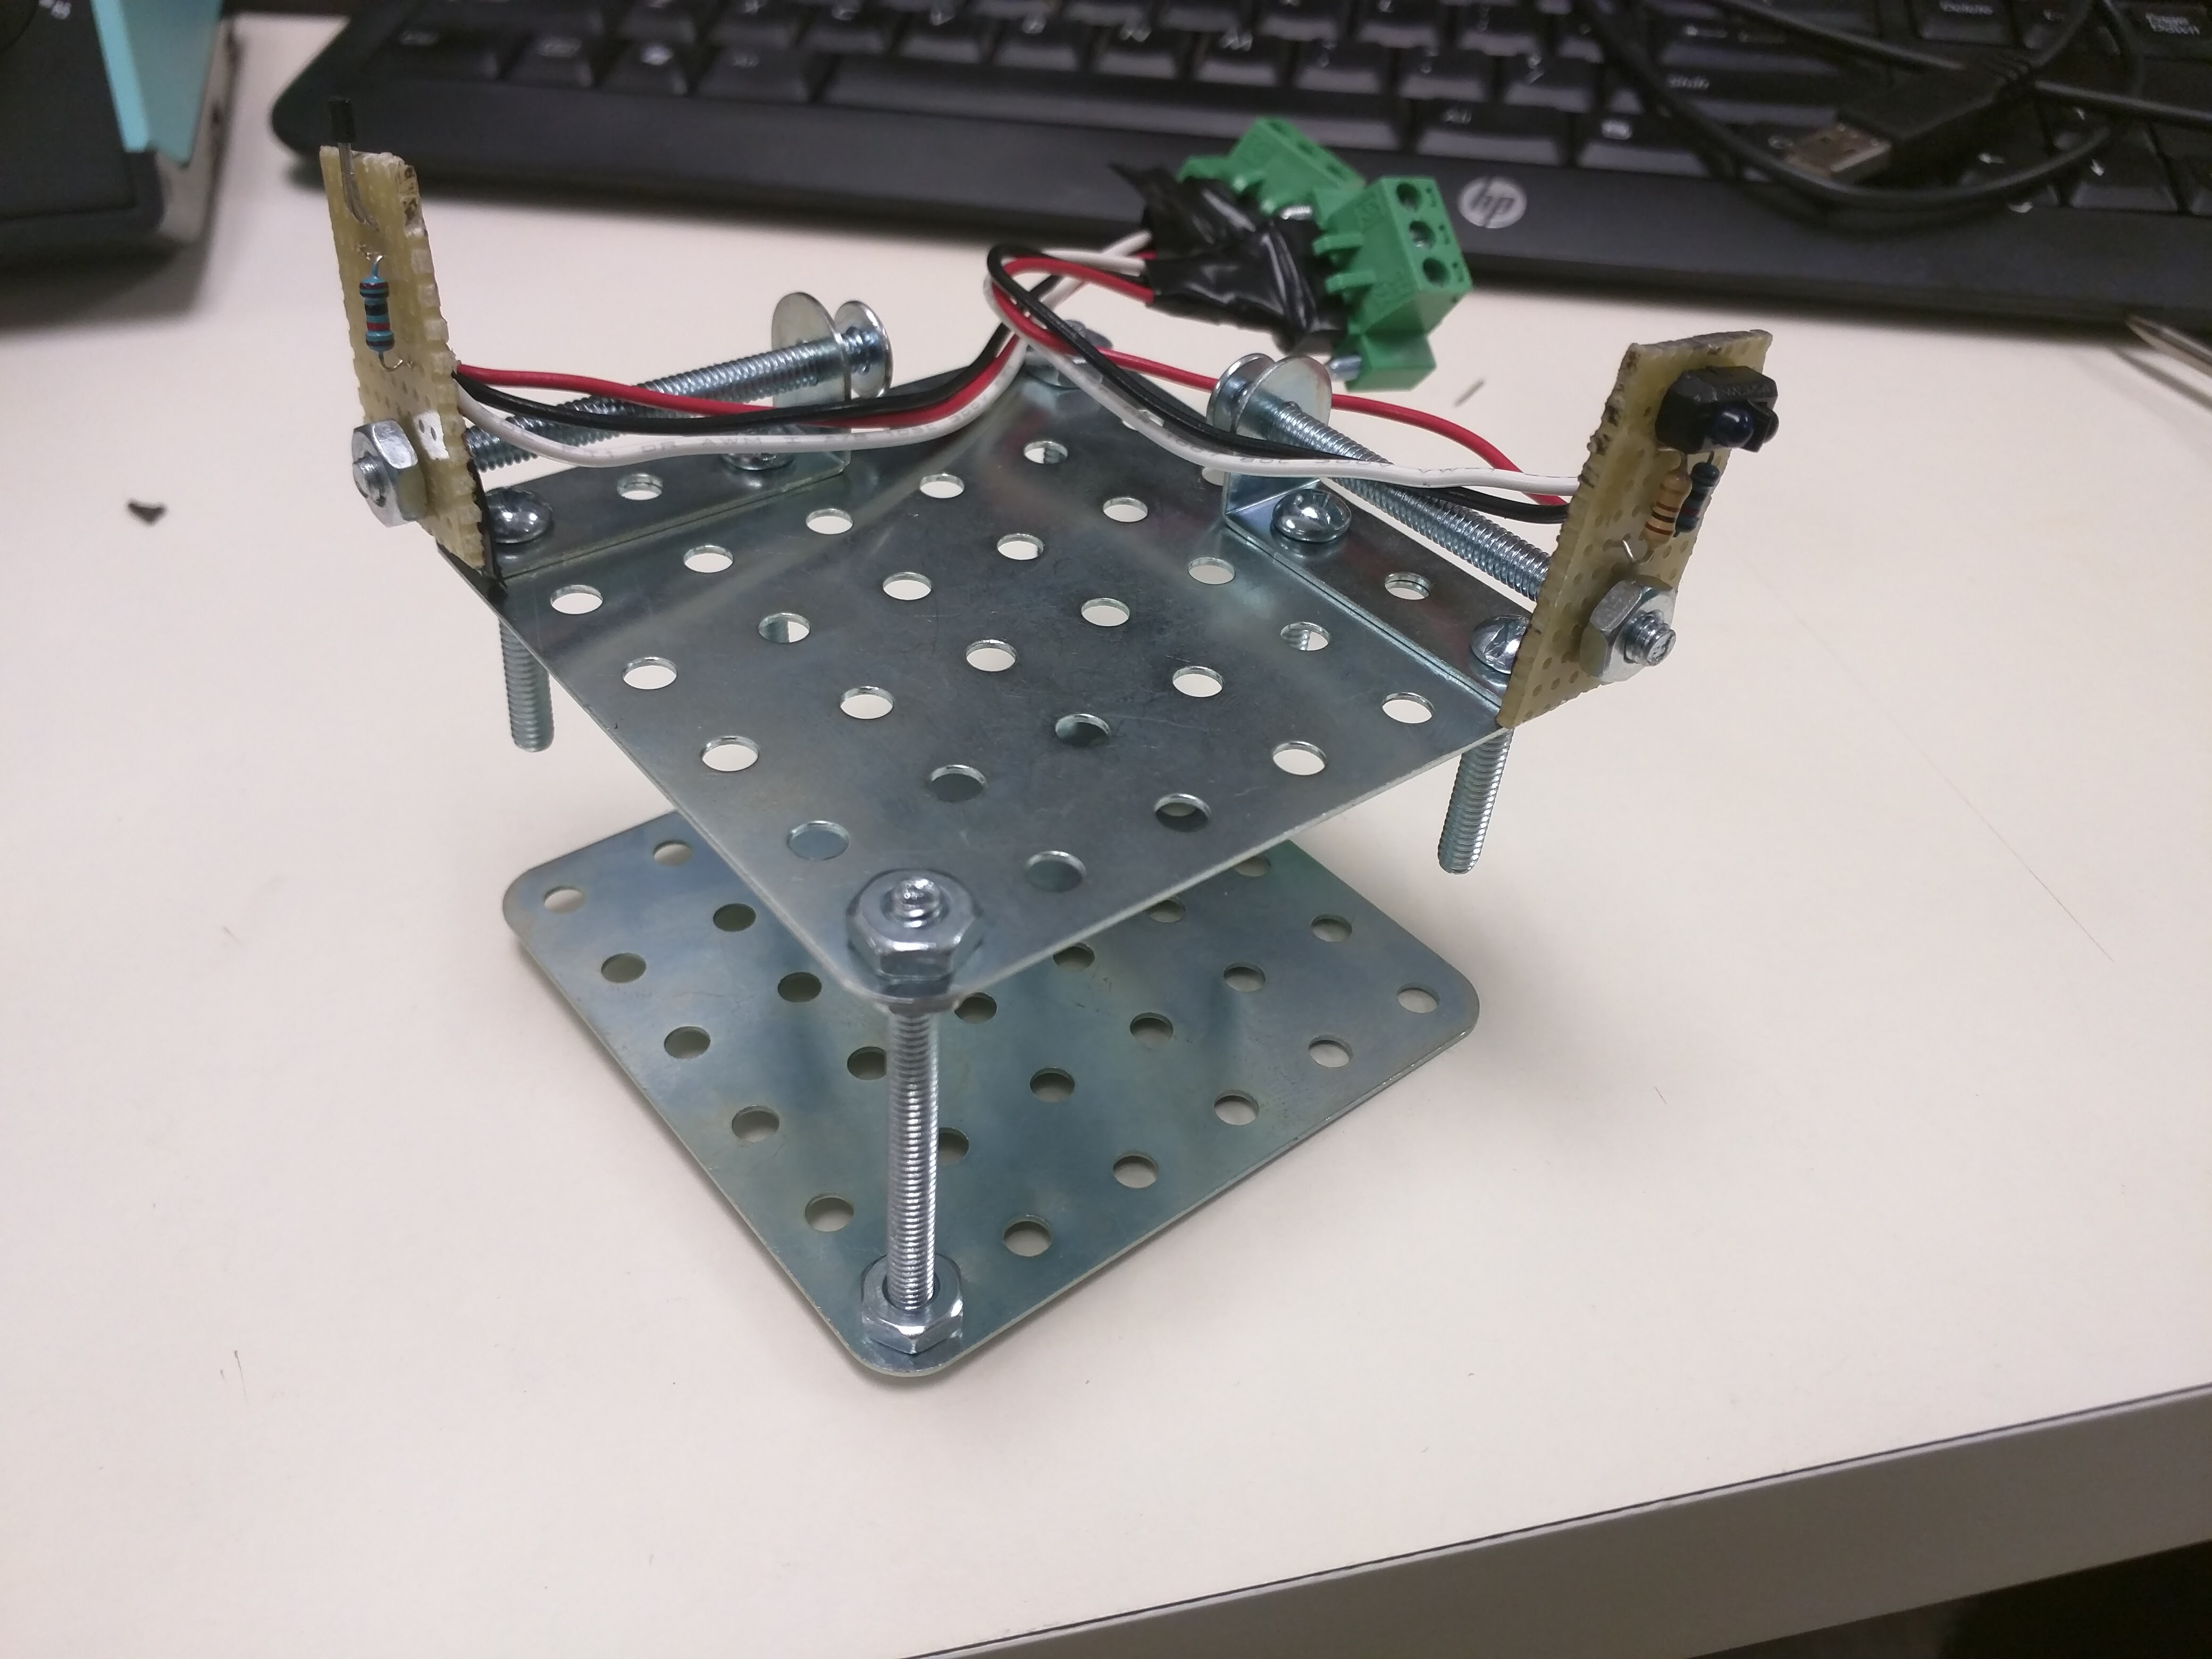
\includegraphics[width=0.5\columnwidth]{figures/prototype.jpg}
    \caption{Two sensors on mounting stage to be installed on observatory wall. Left: hall effect sensor. Right: optical sensor.}
\label{fig:sensors}
\end{figure}
\begin{figure}[h]
    \centering
    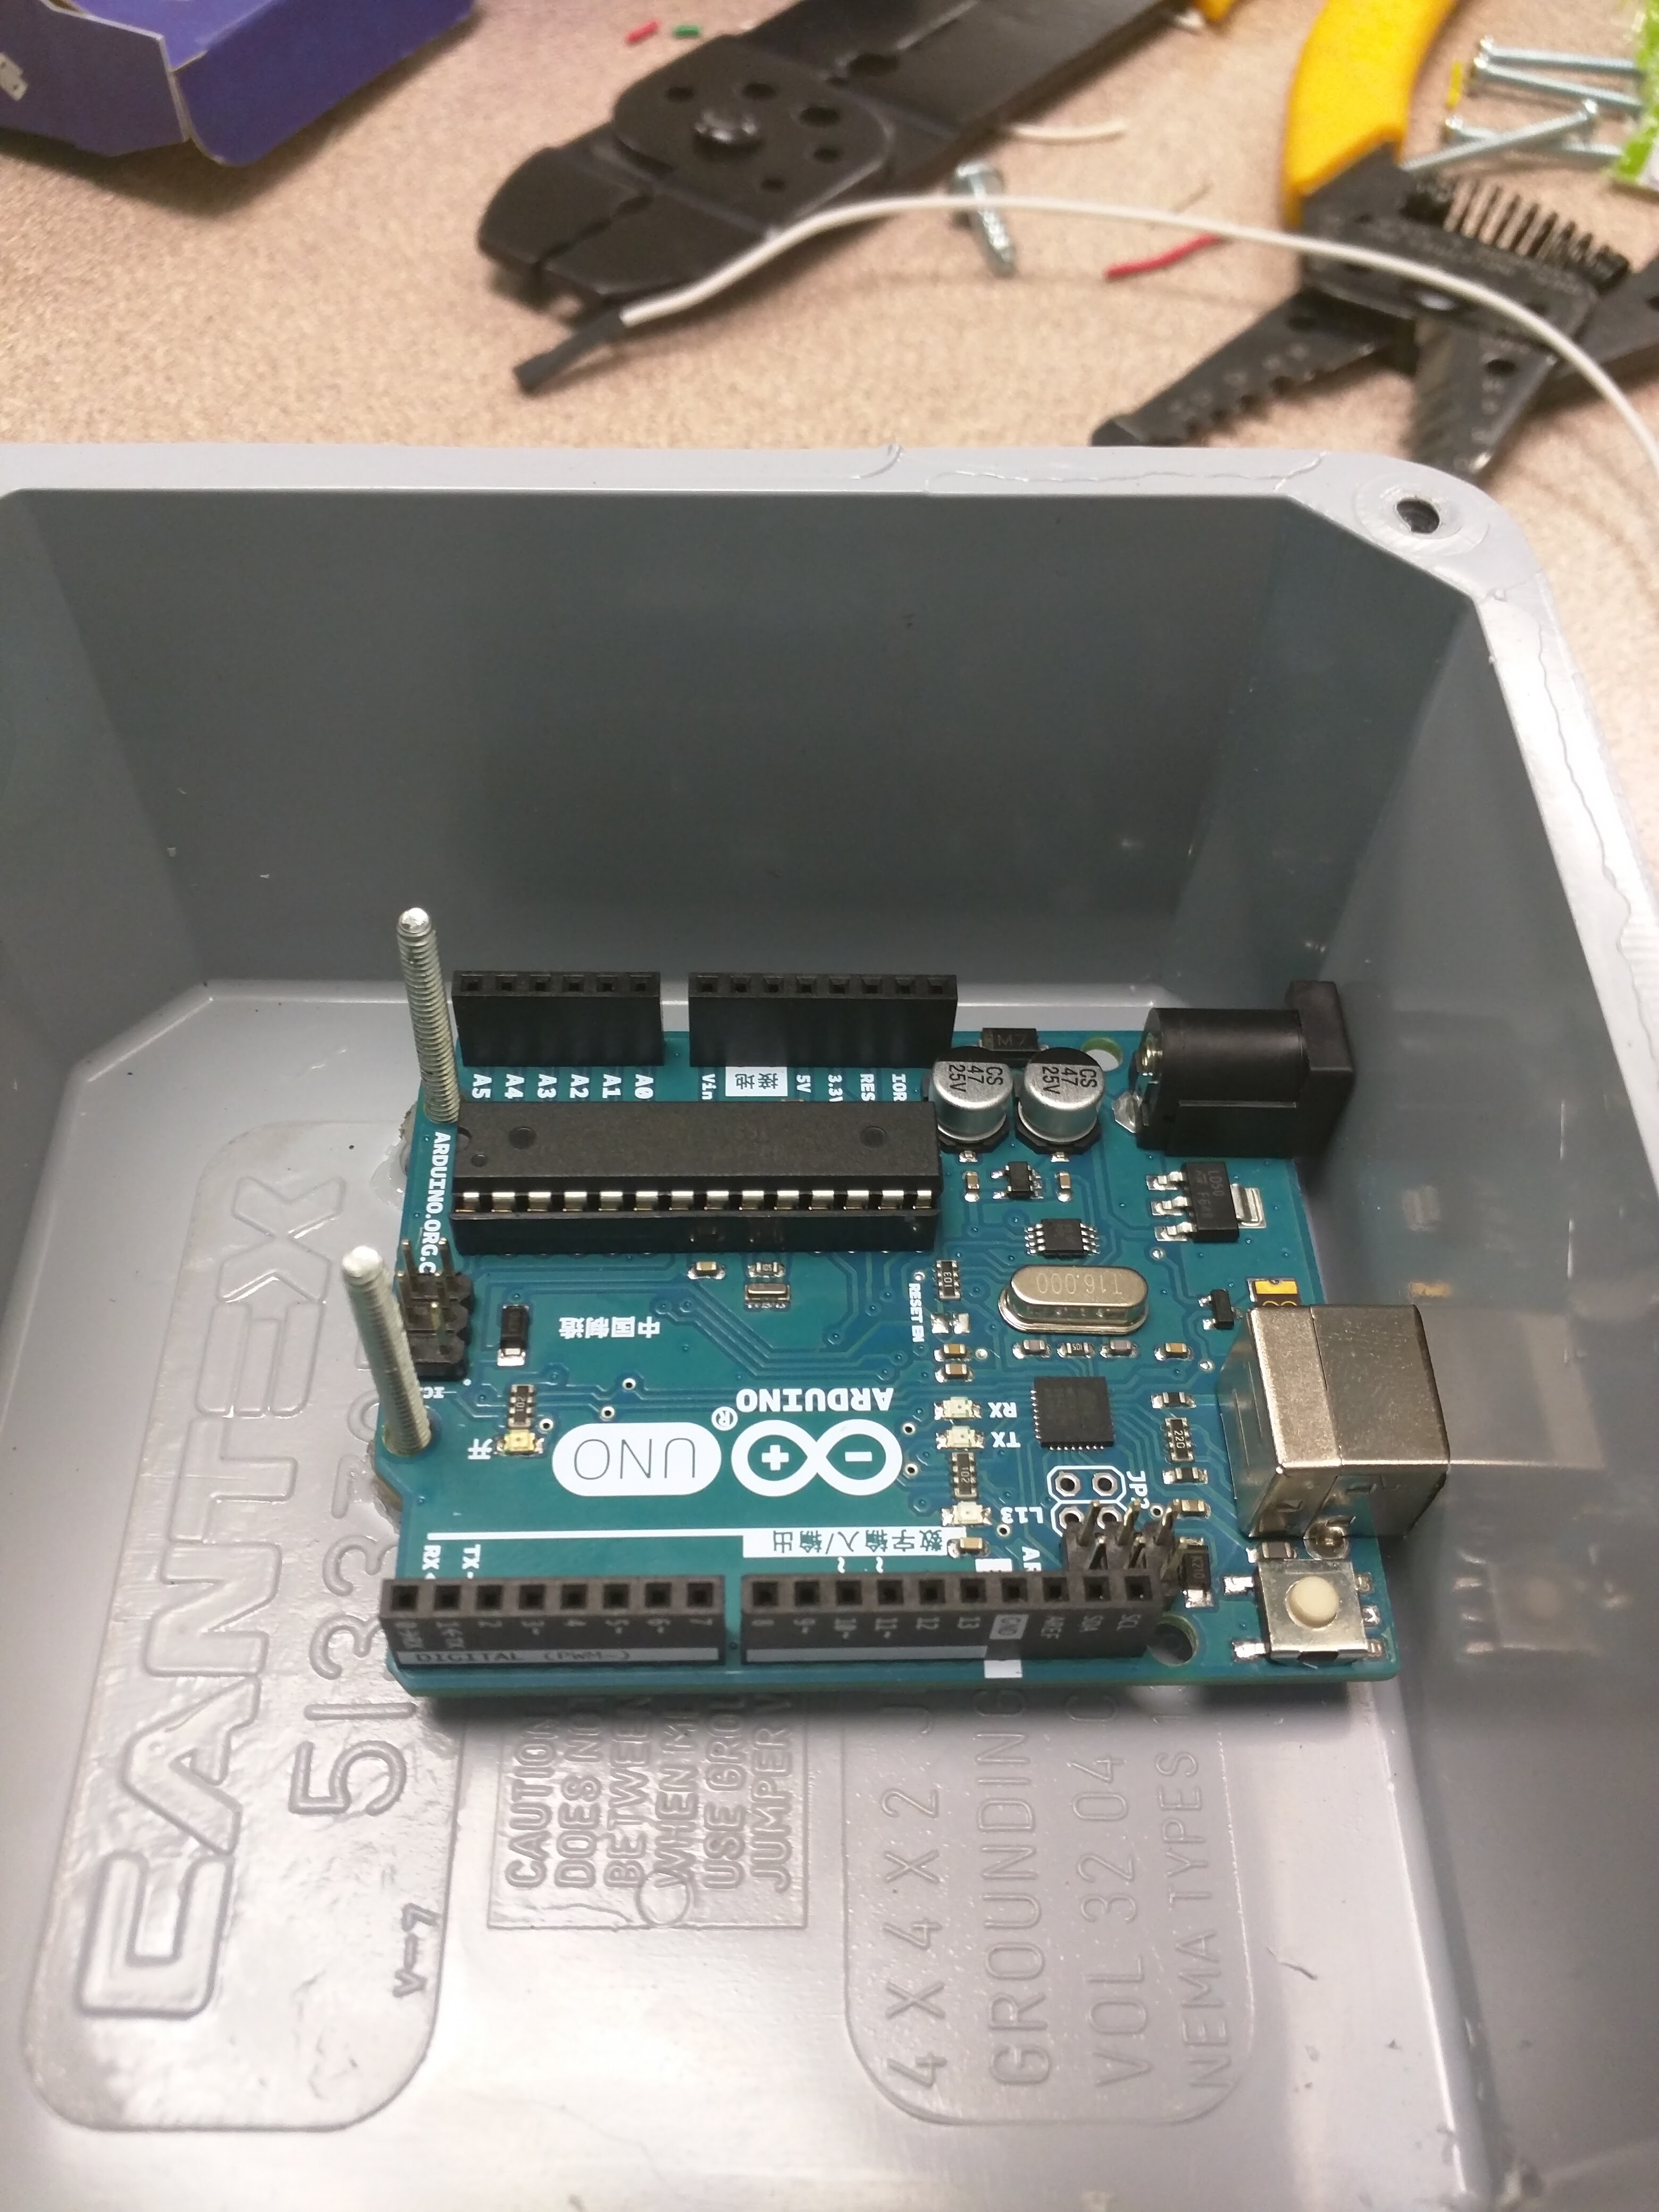
\includegraphics[width=0.5\columnwidth]{figures/arduino.jpg}
    \caption{Arduino Uno inside enclosure}
\label{fig:arduino}
\end{figure}
\begin{itemize}
    \item Dome Rotation
        \begin{itemize}
            \item Arduino Uno  
            \item Yaskawa J1000 Drive
            \item Custom Relay Circuit
        \end{itemize}
    \item Shutter Control Window
        \begin{itemize}
            \item 12 VDC Gel Marine Battery
            \item Custom Controller
        \end{itemize}
    \item Shutter Drawbridge
        \begin{itemize}
            \item Rope
            \item Pulley
        \end{itemize}
\end{itemize}
    
\section{Telescope System}
\subsection{16-inch Meade LX200-GPS}
\begin{figure}[h]
    \centering
    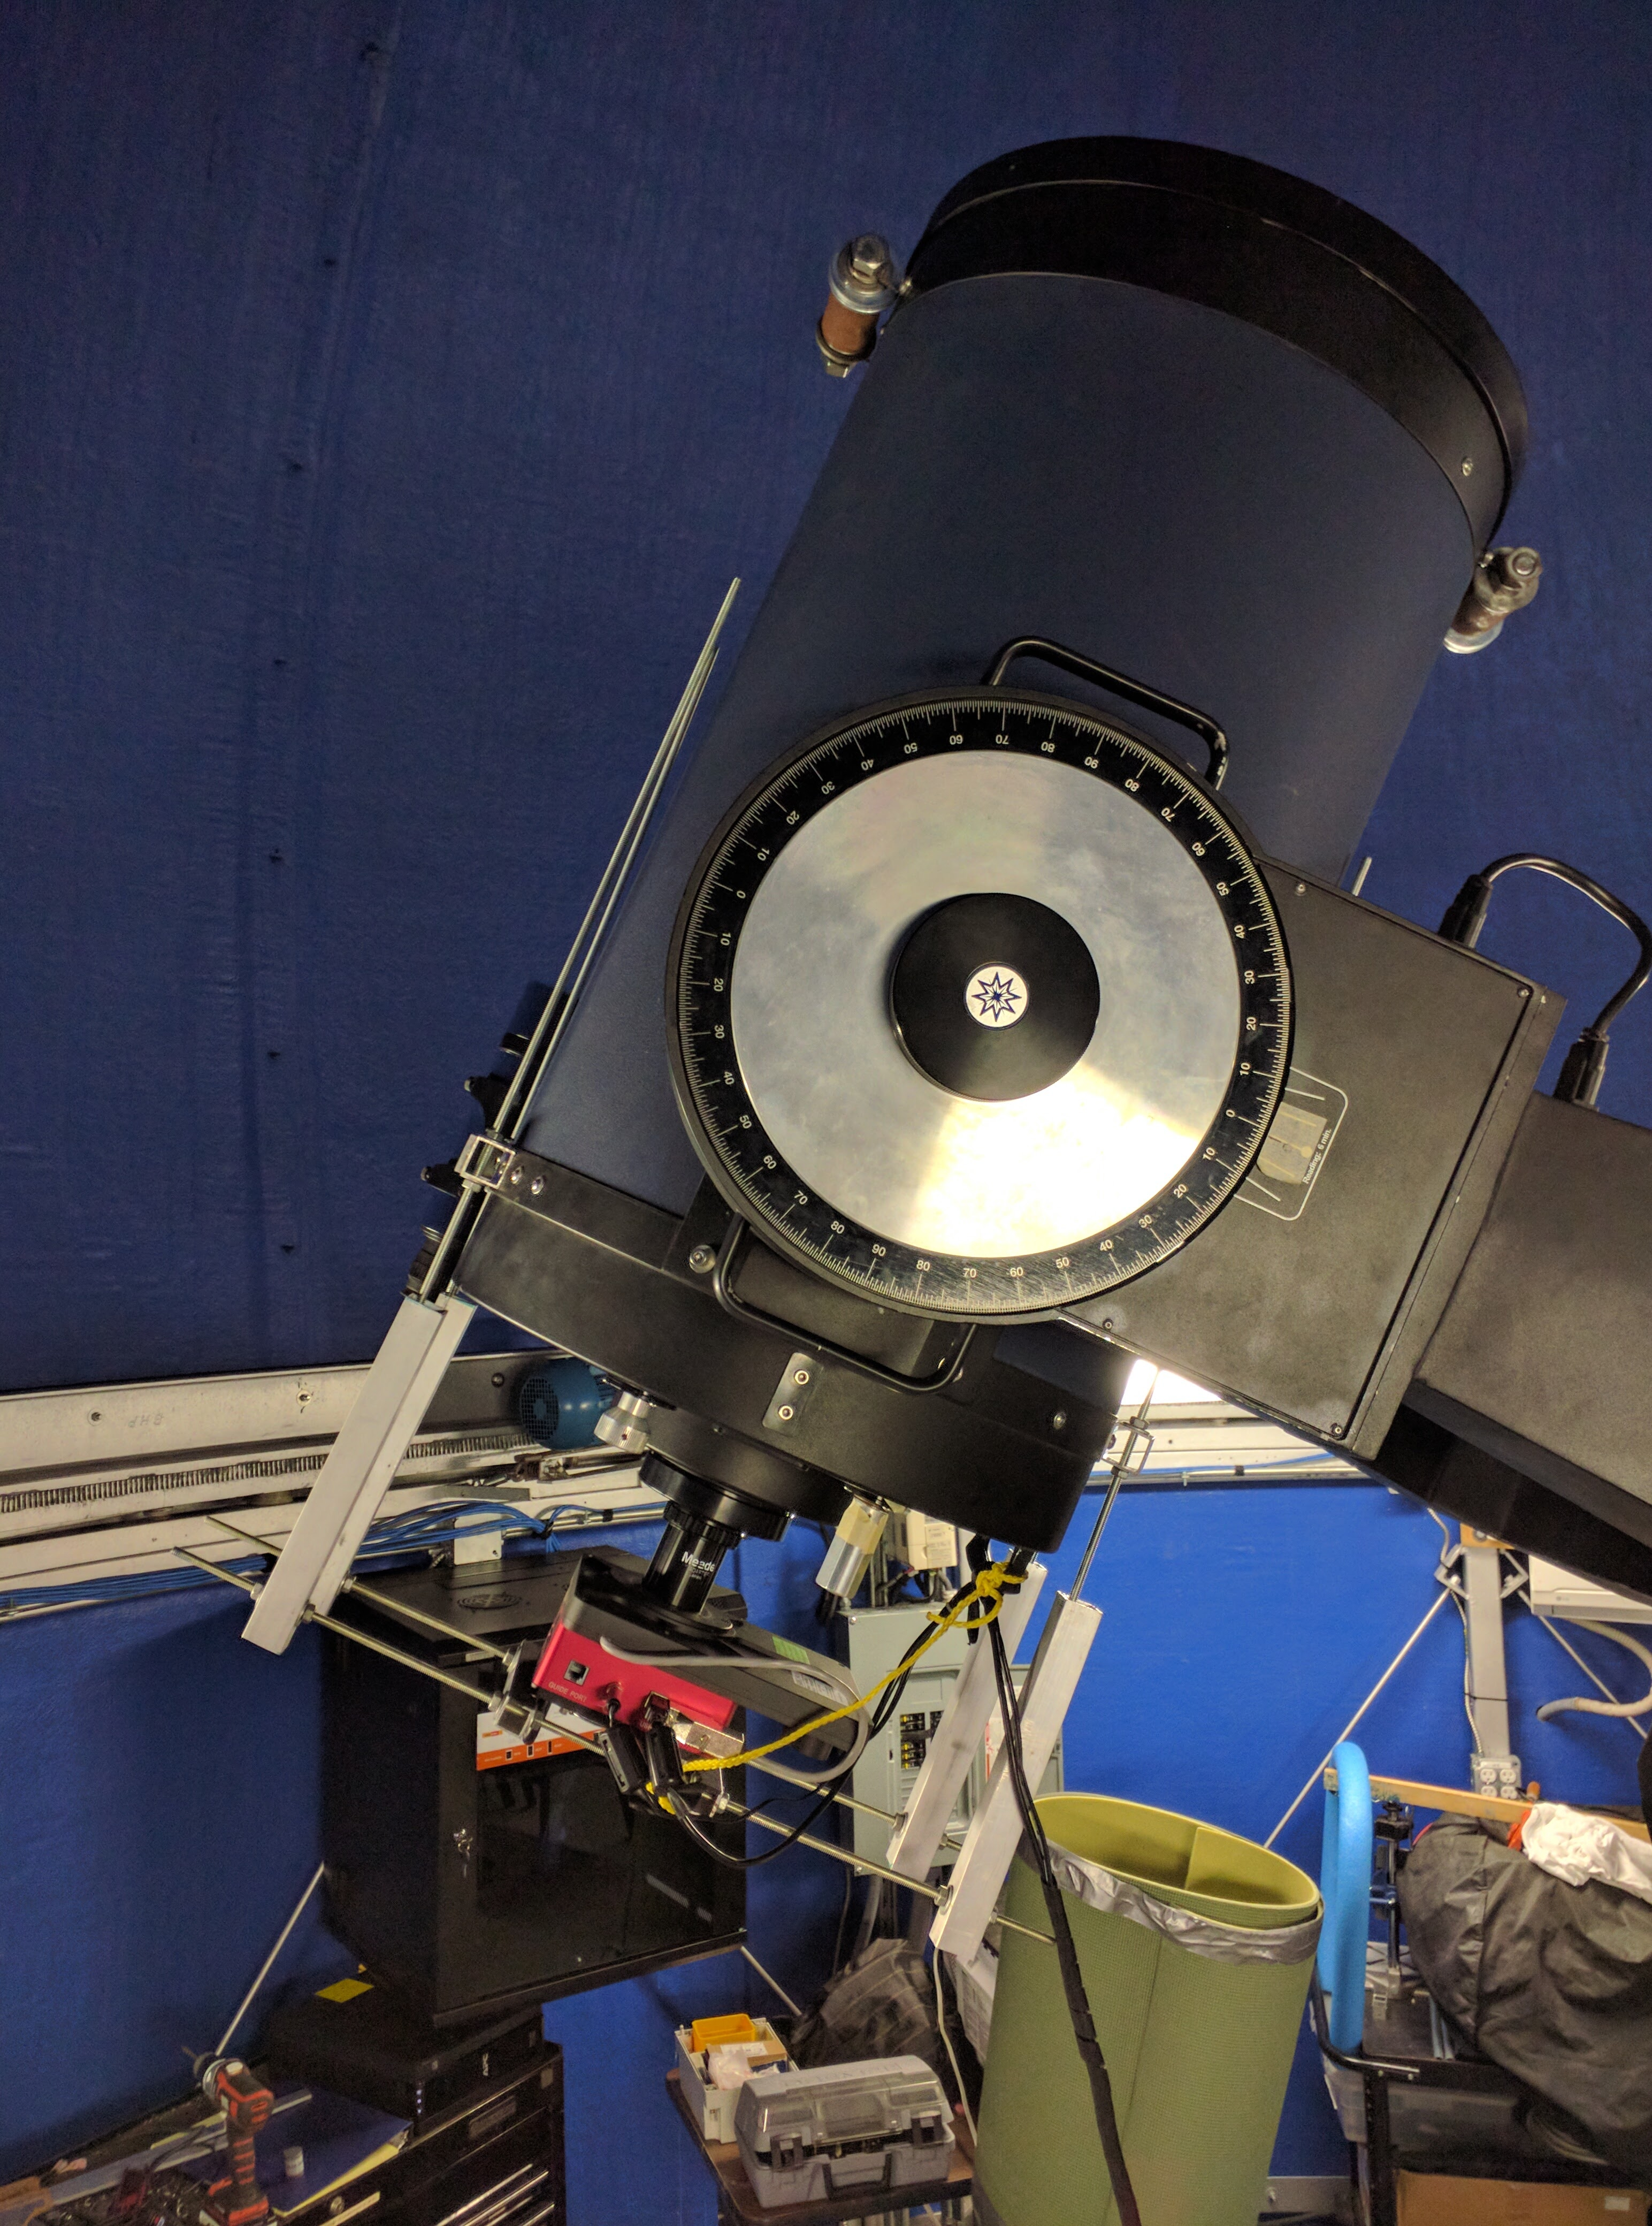
\includegraphics[width=0.5\columnwidth]{figures/meade.jpg}
    \caption{16-in Meade LX200-GPS}
\label{fig:meade}
\end{figure}
\subsubsection{OTA Specifications}
The following specifications are given by the manufacturer Meade Instruments Corporation~\cite{meade_2003} for the optical tube assembly (OTA).
\begin{description}
    \item[Optical design] Schmidt-Cassegrain
    \item[Clear aperture] \SI{406.4}{\milli\meter}
    \item[Focal length] \SI{4064}{\milli\meter}
    \item[Focal ratio] f/10
    \item[Resolving power] \SI{0.28}{\arcsecond}
    \item[Coatings] Meade EMC Super Multi-Coatings
    \item[Mounting] Heavy-duty double-tine forks
    \item[Gears] 11-inch diameter worm gears, both axes
    \item[Periodic error correction] Both axes
    \item[Alignment] Alt-Azimuth or equatorial with optional pier
    \item[Pointing Precision] \SI{2}{\arcminute} in GO TO mode
    \item[Slew Speeds] 1x sidereal to \SI{8}{\deg\per\second} in 9 increments
    \item[Power] 18V power supply
    \item[Accesories] These are devices used during regular observations or setup
        \begin{itemize}
            \item 8x \SI{50}{\milli\meter} viewfinder
            \item 4-speed zero image-shift microfocuser
            \item 16-channel GPS receiver
            \item True-level electronic sensor
        \end{itemize}
    \item[Net telescope weight] 110 lbs
\end{description}

\subsubsection{Telescope Pier}
Telescope pier was constructed by a custom pedestal and the optional equatorial wedge made by Meade.
\begin{description}
    \item[Pedastal height] 44.25 inches
    \item[Wedge height] 32 inches
    \item[Wedge inclination] \SI{26}{\deg}
    \item[Weight] 225 lbs
\end{description}

\subsubsection{Installation}
Installation required multiple steps.
First, using a chain winch we set the pedestal onto bolts that were installed in the base of the concrete pad designed for the load of the telescope. 
Second, using the winch we installed the pier on top of the pedestal keeping alignment of the wedge due north for polar alignment of the telescope.
Third, using the winch we lifted the telescope to the wedge and bolted the instrument.

A special bolting technique was used to allow for precise polar alignment.

\subsubsection{Limitations}
Exposures longer than 30 seconds were not possible due to noticeable drift.
Attempts were made to correct for this issue by doing a drift polar alignment.

The microfocuser was not able to hold the weight of the cameras used for research.
The author designed and constructed a rig pictured in figure~\ref{fig:rig} that fit on the back of the OTA that supported the extra weight and allowed
for regular function of the microfocuser.
\begin{figure}[h]
    \centering
    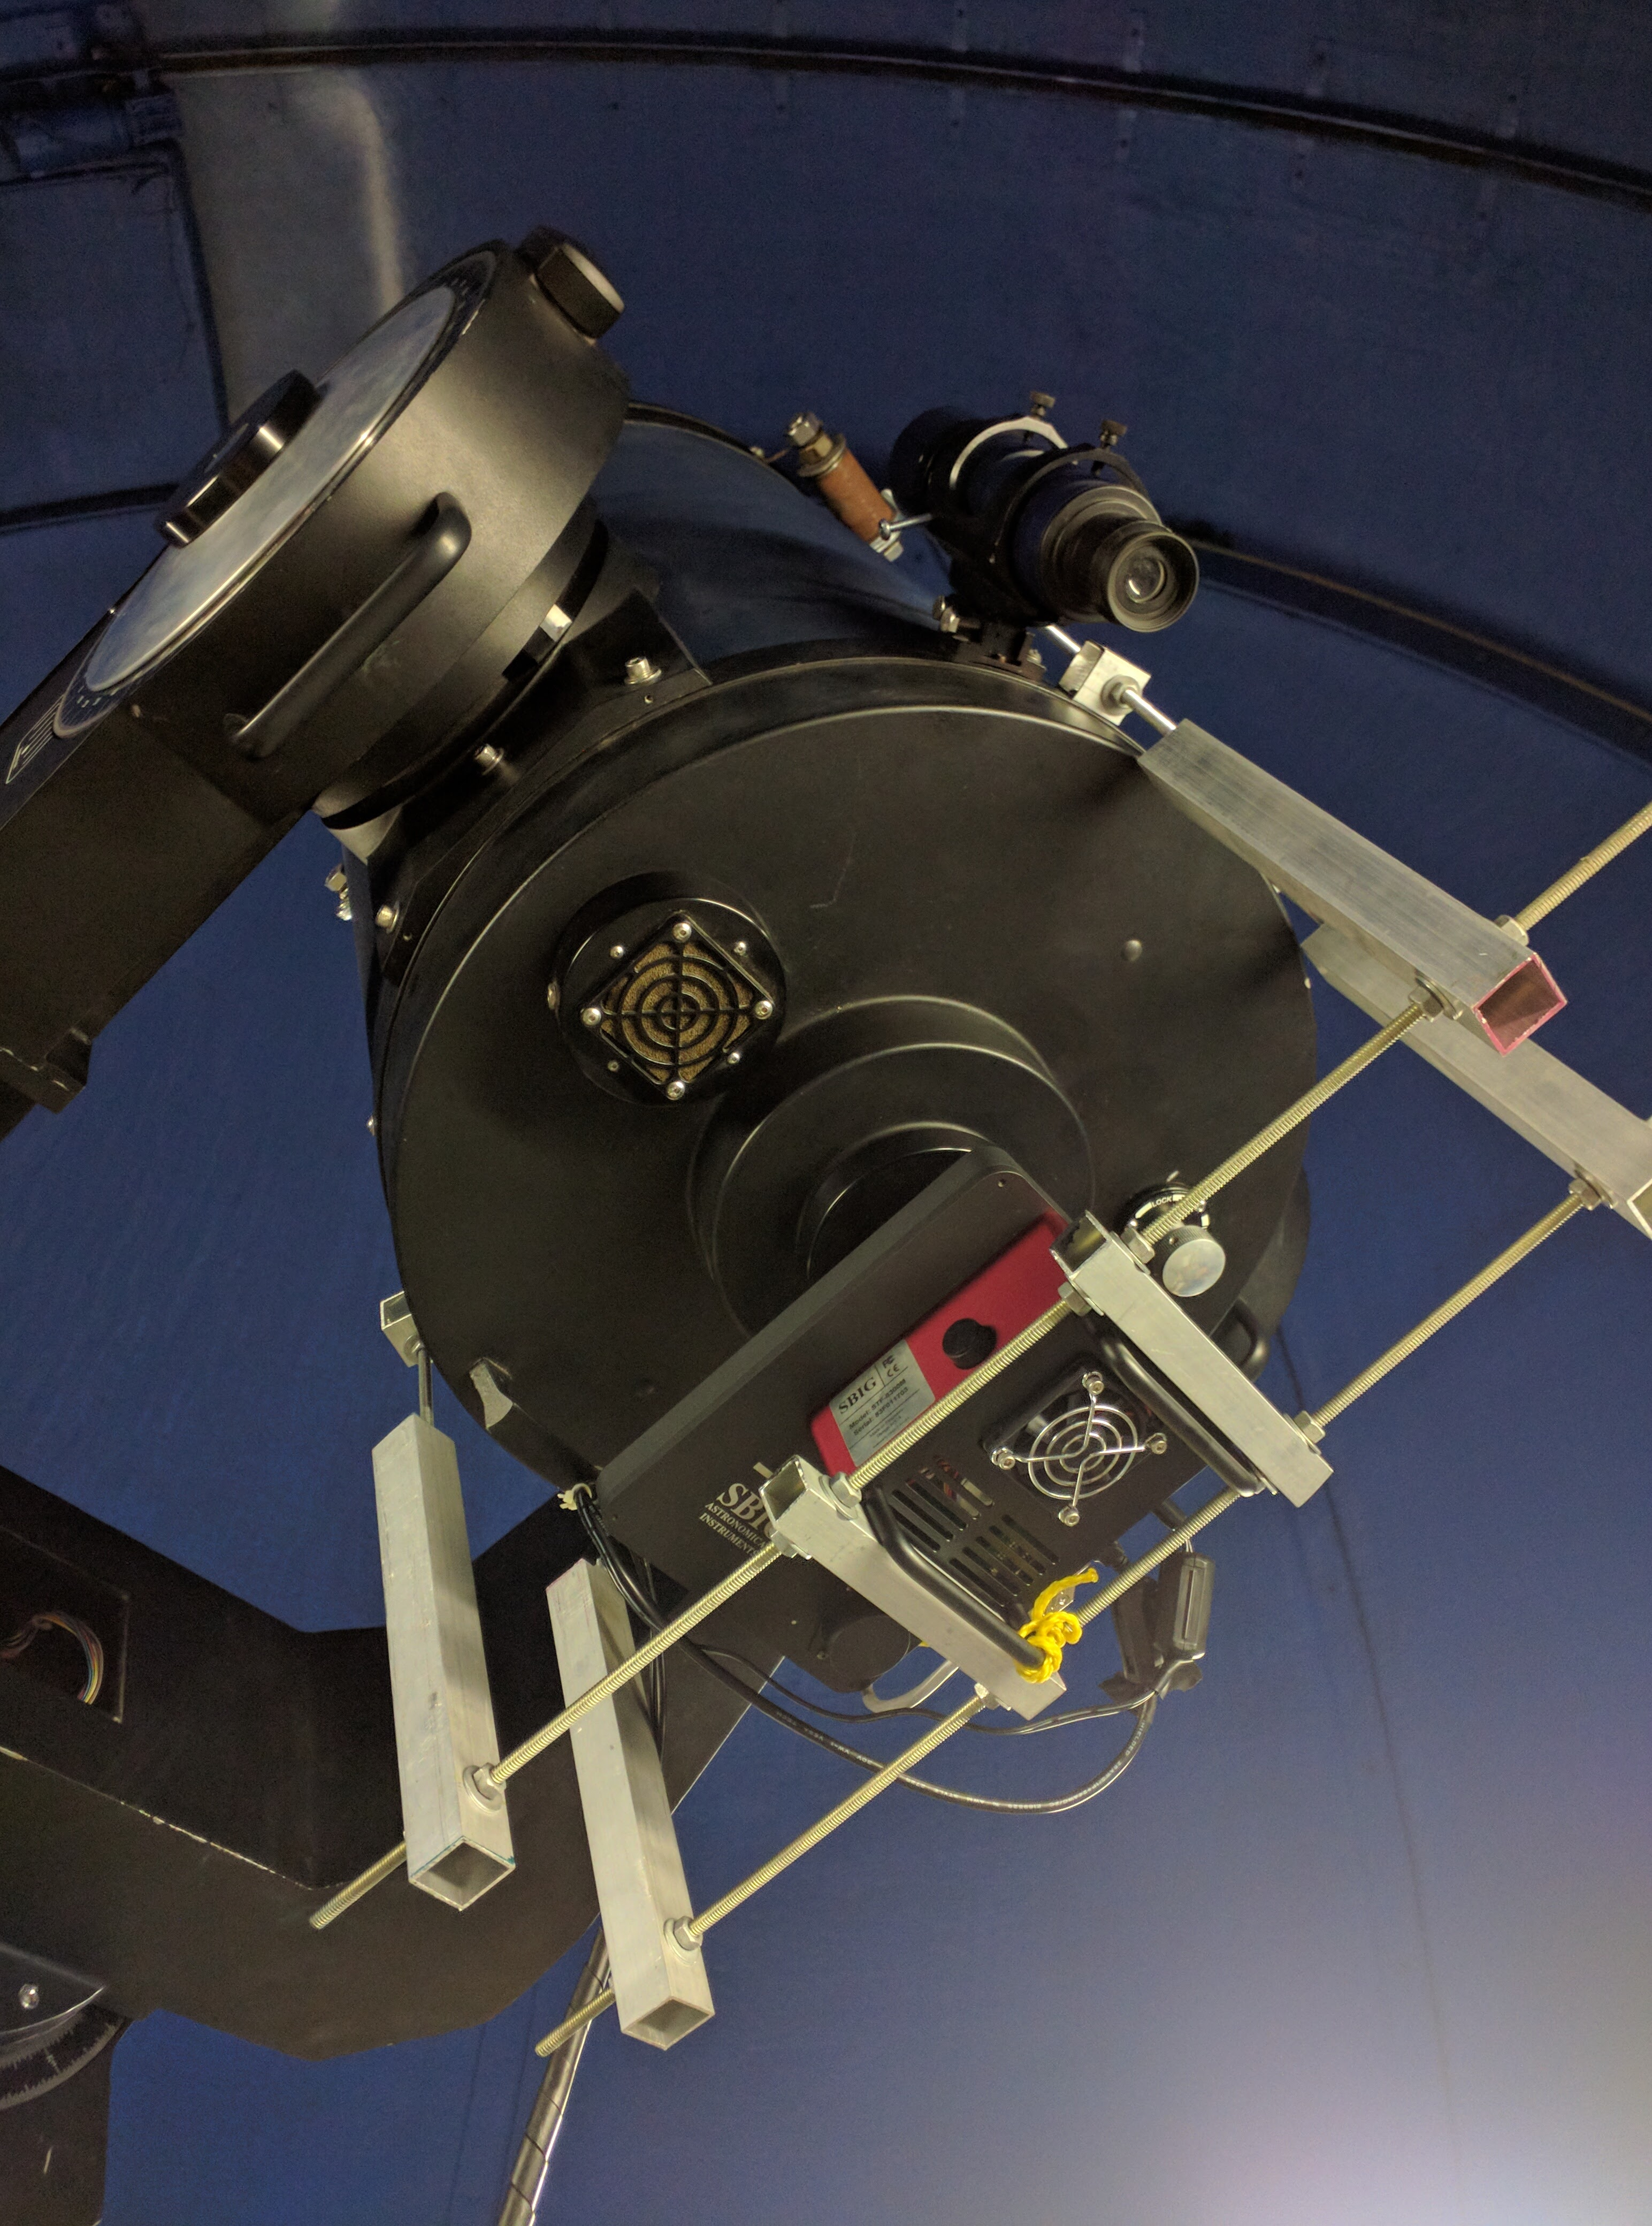
\includegraphics[width=0.5\columnwidth]{figures/rig.jpg}
    \caption{Rig that was designed and constructed by the author shown supporting SBIG STF8300 behind 16-in Meade LX200-GPS}
\label{fig:rig}
\end{figure}

% According to the aperture of the telescope, an ideal limiting magnitude is calculated, assuming perfect optics, camera, and sky brightness,
% i.e.\  spacelike conditions.
% The estimation for limiting flux of a space based telescope as explained by Chromey~\cite{chromey_2010} is given by,
% \begin{equation}
%     f_{\text{d,space}} = {\left(\frac{h c\lambda}{Q}\right)}^\frac{1}{2} {\left( \frac{b_{\lambda}}{t}\right)}^\frac{1}{2}\frac{2.44}{D^2}
%     \label{eq:limflux}
% \end{equation}
% where the first term refers to the quantum efficiency of the camera, the second term refers to
% the sky brightness over the exposure time, and the last term assumes telescope is
% diffraction limited\footnote{Diffraction limited refers to an optical system at its theoretical limit.}.
% 
% To convert from flux, $f$, to magnitude, $m$, we use the following equation,
% \begin{equation}
%     m = -2.5 \log{f}
%     \label{eq:flux2mag}
% \end{equation}
% and find the limiting magnitude to be 12.
% 
\subsection{CDK17 on L-500 direct drive mount}
\subsubsection{Specifications}
The following specifications are given by the manufacturer PlaneWave Instruments~\cite{cdk17} for the optical tube assembly (OTA).
\begin{description}
    \item[Optical design] Corrected Dall-Kirkham
    \item[Aperature] \SI{432}{\milli\meter}
    \item[Focal length] \SI{2939}{\milli\meter}
    \item[Focal ratio] F/6.8
    \item[OTA Weight] 106 lbs
    \item[OTA length] \SI{1067}{\milli\meter}
    \item[Feature] Three cooling fans ejecting air from the back of the telescope and four fans blowing across the boundary layer of the mirror surface. This helps the telescope to reach thermal equilibrium quickly. The fans are controlled by a computer if the optional Electronic Focus Accessory (EFA Kit) is purchased.
    \item[Mounting] L-500 direct drive mount
    \item[Mount weight] 257 lbs
    \item[Load Capacity] 200 lbs
    \item[Slew Rate] 20 degrees per second (standard); 50 degrees per second (maximum), both axes
    \item[Motor Control] Industrial grade brushless motor control system and built in electronics
    \item[Pointing Accuracy] $<10$ arcsecond RMS with PointXP Model
    \item[Pointing Precision] 2 arcsecond
    \item[Tracking Accuracy] $< 0.3$ arcsecond error over 5 minute period
    \item[System Natural Frequency] 10 Hz or greater
    \end{description}

\subsubsection{Telescope Pier}
The manufacturer Planewave Instruments provided a tool for calculating the required pier height for their wedge and L-500 Direct Drive Mount.
We used the same pedestal that was used with the Meade pier.
\begin{figure}[h]
    \centering
    \includegraphics[width=0.5\columnwidth]{figures/pier.jpg}
    \caption{Pedestal, pier, and wedge before installation of mount}
\label{fig:pier}
\end{figure}
\begin{description}
    \item[Pedastal height] 44.25 inches
    \item[Wedge inclination] for latitudes 22--28 degrees
    \item[Wedge weight] 145 lbs
    \item[Pier height] 12 inches
\end{description}

\subsubsection{Installation}
\begin{figure}[h]
    \centering
    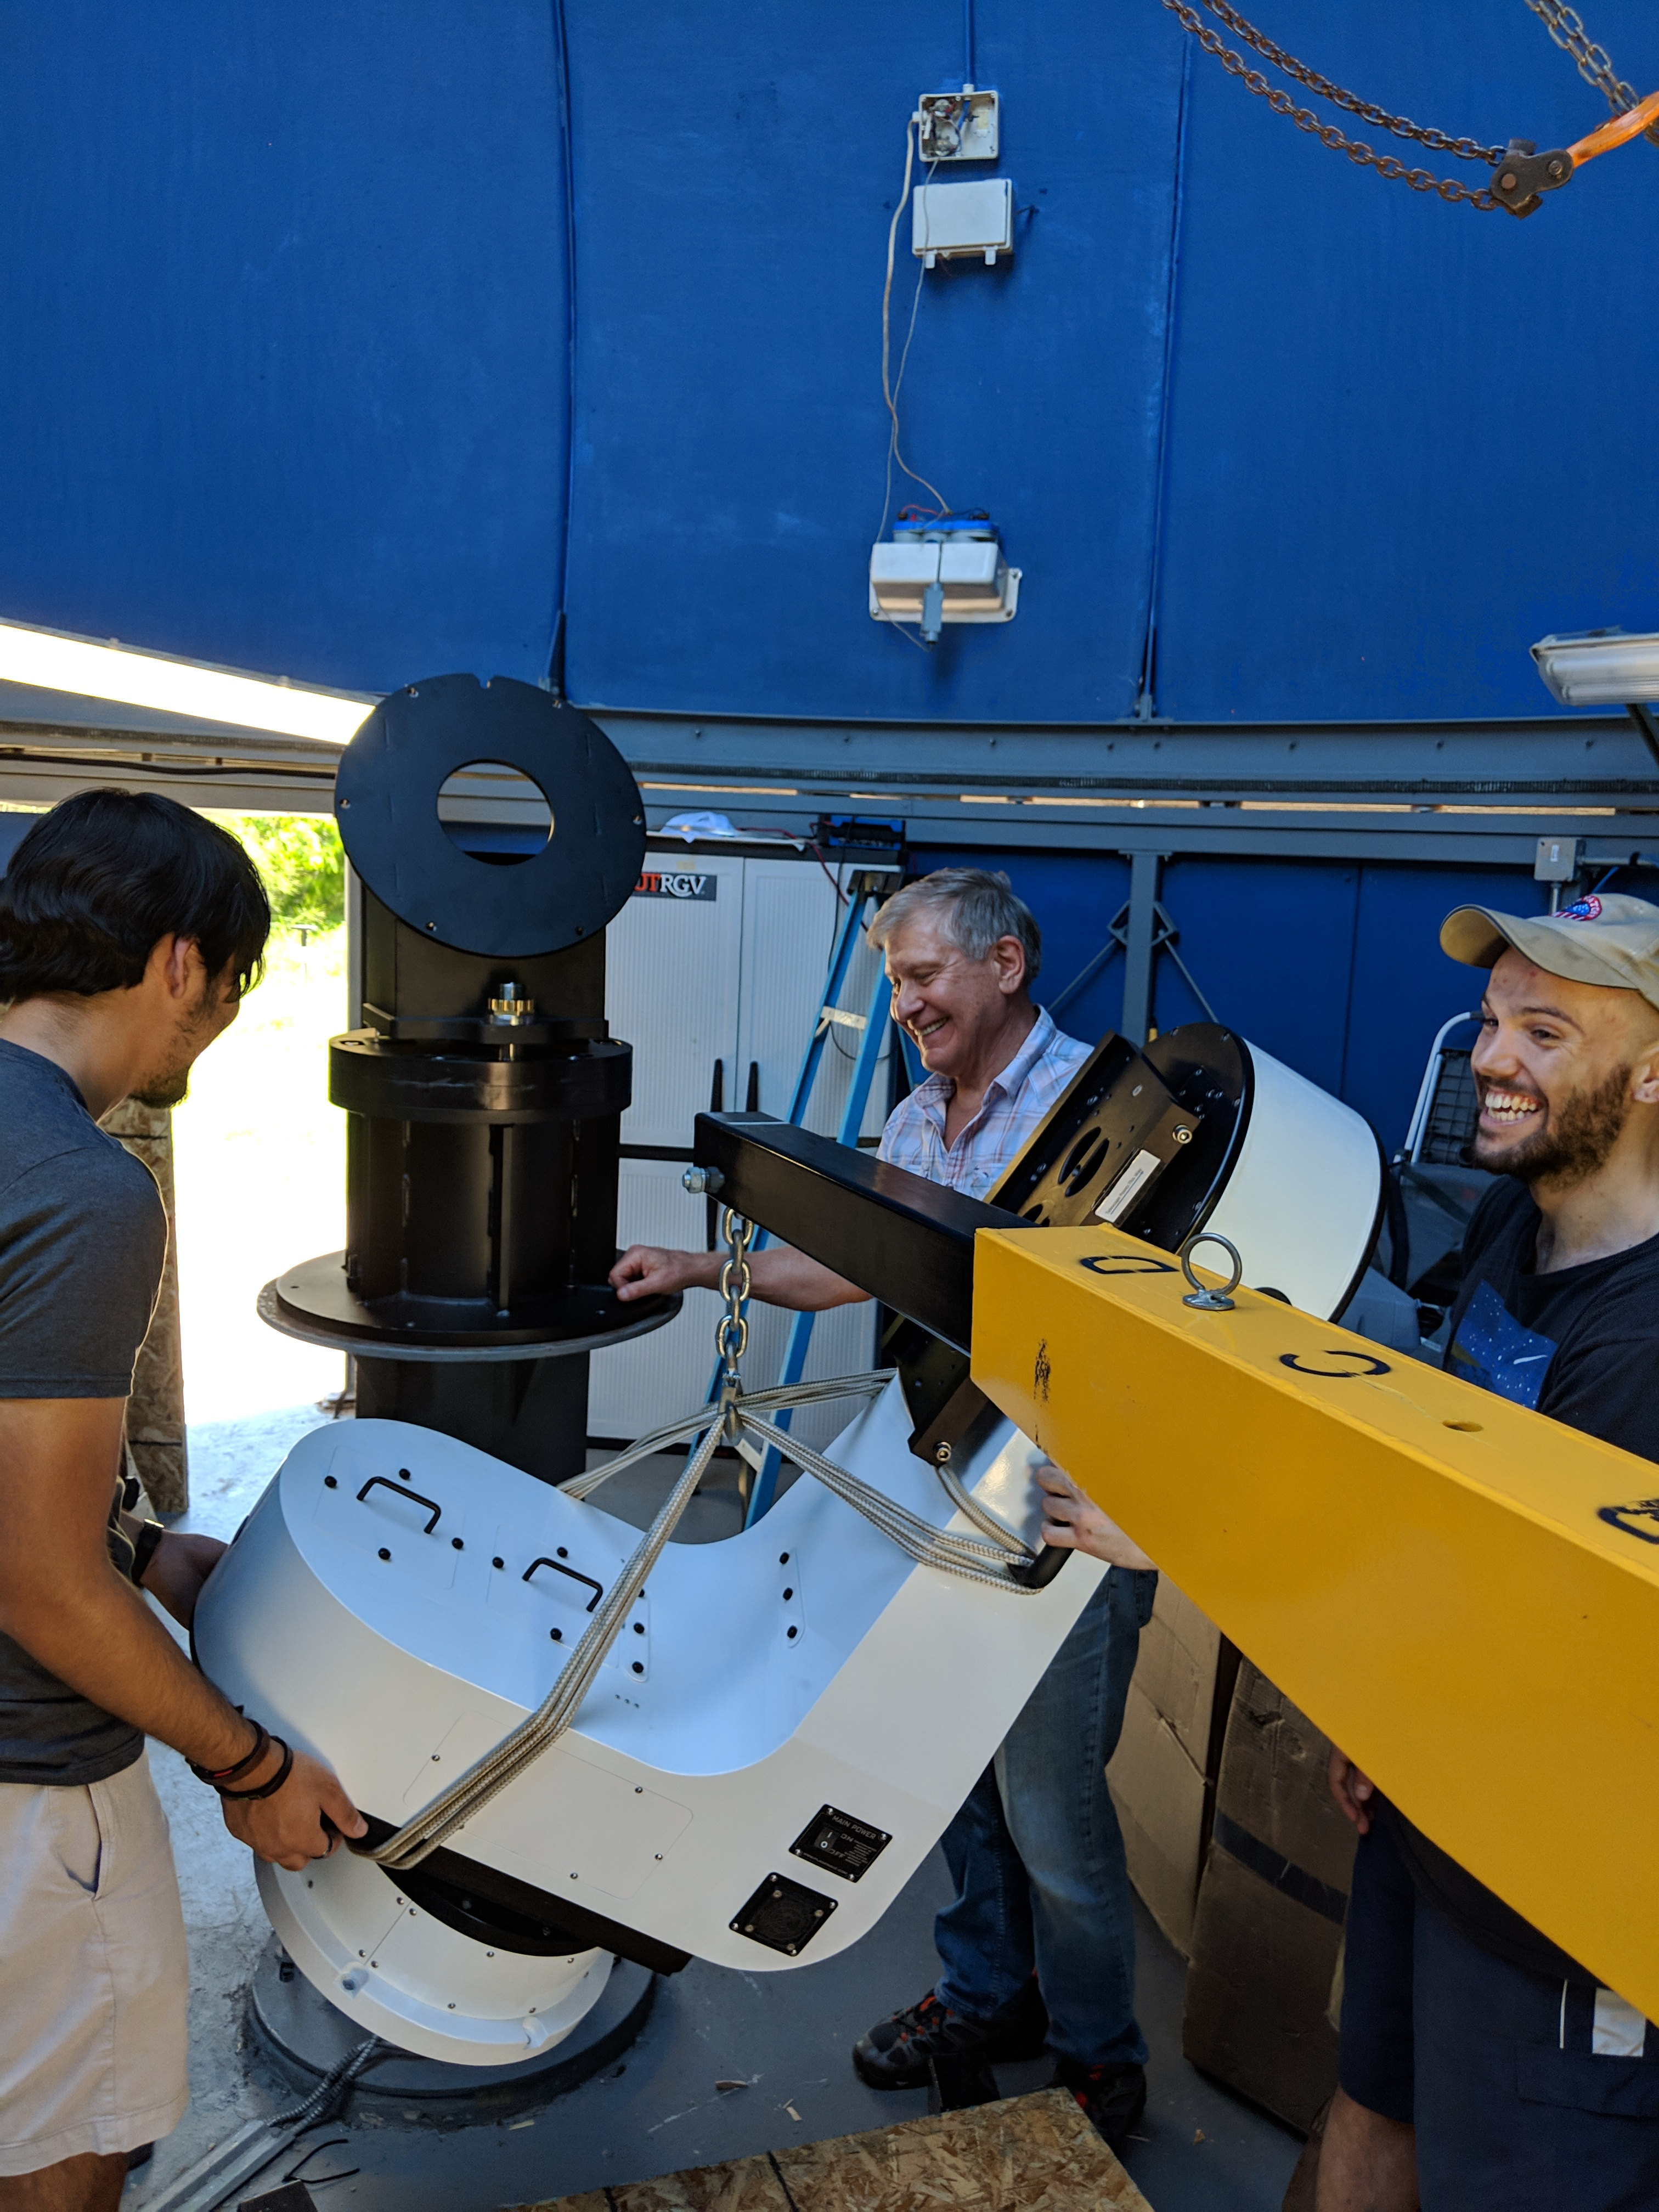
\includegraphics[width=0.5\columnwidth]{figures/cdkinstall.jpg}
    \caption{Installation of CDK500}
\label{fig:cdkinstall}
\end{figure}
The installation of the CDK17 with L-500 mount required the removal of the 16-inch Meade LX200 GPS Telescope system and wedge from the pedestal.
After removal of the Meade system, we installed the 12-inch pier on the pedestal.
Over the pier we installed the wedge and did a rough alignment to due north for polar alignment.
Precision was not critical at this point since the Planewave wedge for L500 mount features fine latitude and azimuth adjustments.
We used a combination of a winch and motor hoist crane to support the weight of the L-500 mount to bolt the mount to the wedge.
Finally, we adjusted the saddle of the telescope and fit onto the mount.

Prior to use, balancing was done with the camera and focuser installed.
The manufacturer had to remotely recalibrate the motors due to the weight of instrumentation.

Pointing model is required for proper pointing. This was created following a process in PWI3, software developed by Planewave.
First, 30 evenly spaced point above 30 degrees in altitude were selected. 
The software commands the telescope to one of 30 points, takes a picture,
finds the positions of all objects in the frame through a process called plate solving to establish precise pointing position, and
updates the table of the pointing to the plate solved position.

\subsubsection{Limitations}
%Using equations~\ref{eq:limflux} and~\ref{eq:flux2mag}, we find the diffraction limited telescope limiting magnitude to be 12.2.
We have found no issues with drifting with exposures longer than 2 minutes and tracking holding steady for over 4 hours.

\section{Camera}
\subsection{Pixel Scale}
Pixel scale is a conversion between the angular distance of sky that is visible per pixel.
Chromey~\cite{chromey_2010} describes pixel scale as,
\begin{equation}
    \text{pixel scale} = \frac{206,265}{f} d
    \label{eq:pixelscale}
\end{equation}
where $f$ is the focal is the focal length and $d$ is the separation between the centers of pixels.
For our calculations, we will assume $d$ is equal to the pixel width.

\subsection{Field of View}
Field of view (FOV) refers to the angular distance of sky that is visible through the telescope given the physical parameters of the CCD\@.
FOV can be calculated by the following equation as described by Chromey~\cite{chromey_2010},
\begin{equation}
    \text{FOV} = (\text{pixel scale})(\text{length}) \times (\text{pixel scale})(\text{width})
    \label{eq:fov}
\end{equation}

\subsection{SBIG STF-8300}
The following specifications are given by the manufacturer Diffraction Limited~\cite{sbig}.
\subsubsection{Specifications}
\begin{description}
    \item[CCD] Kodak KAF-8300
    \item[Pixel Size] $5.4 \times \SI{5.4}{\micro\meter}$
    \item[Pixel Array] $3326 \times 2504$ pixels
    \item[CCD Size] $17.96 \times \SI{13.52}{\milli\meter}$
    \item[Gain] $\SI{0.37}{\elementarycharge-\per\text{ADU}}$
    \item[Read noise] $\SI{9.3}{\elementarycharge}$
    \item[Digitization Rates] 10 Megapixels / Second
    \item[Full Frame Download] Less than 1 second
    \item[Weight] 1.8 pounds
\end{description}
Linearity tests of the SBIG STF-8300 have been performed and documented by Camuccio~\cite{richard_2019a} to measure gain and read noise.
A plot of the mean pixel value vs the exposure time is show in figure~\ref{fig:linearitysbig}.
\begin{figure}[h]
    \centering
    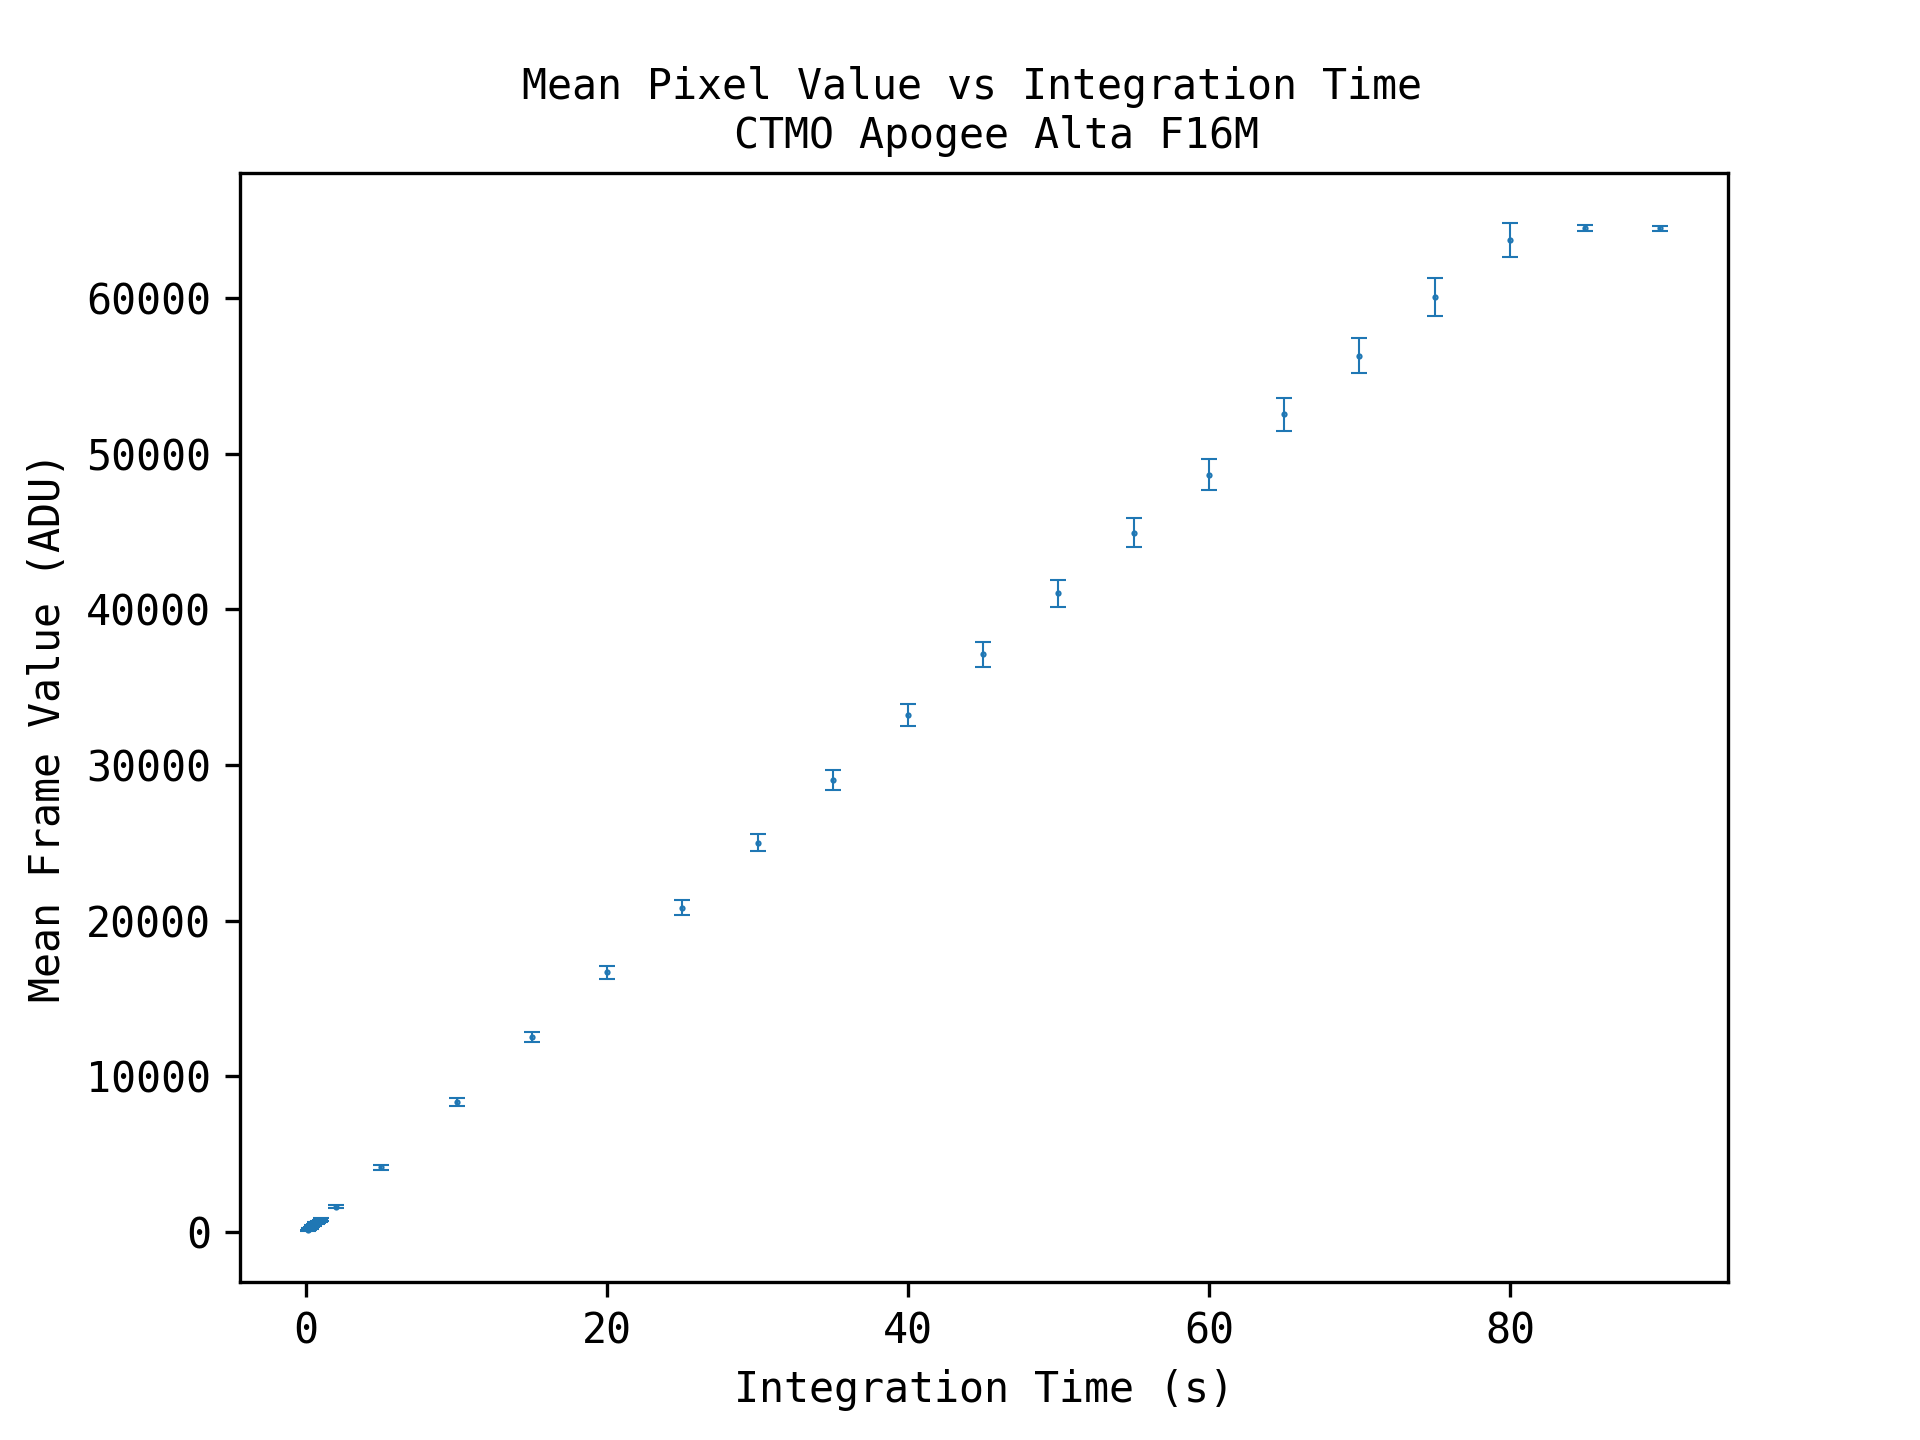
\includegraphics[width=\columnwidth]{figures/sbig_linearity.png}
    \caption{Linearity test of SBIG SFT-8300 performed by Richard Camuccio~\protect\cite{richard_2019a}}
\label{fig:linearitysbig}
\end{figure}

\subsubsection{16-inch Meade}
Using equations~\ref{eq:pixelscale} and~\ref{eq:fov} to find pixel scale and FOV, respectively, we find, 
\begin{description}
    \item[Pixel scale] \SI{0.274}{\arcsecond\per\text{pixel}}
    \item[FOV] $\SI{15.19}{\arcminute} \times \SI{11.44}{\arcminute}$
\end{description}

\subsection{Apogee Alta F16M}
\begin{figure}[h]
    \centering
    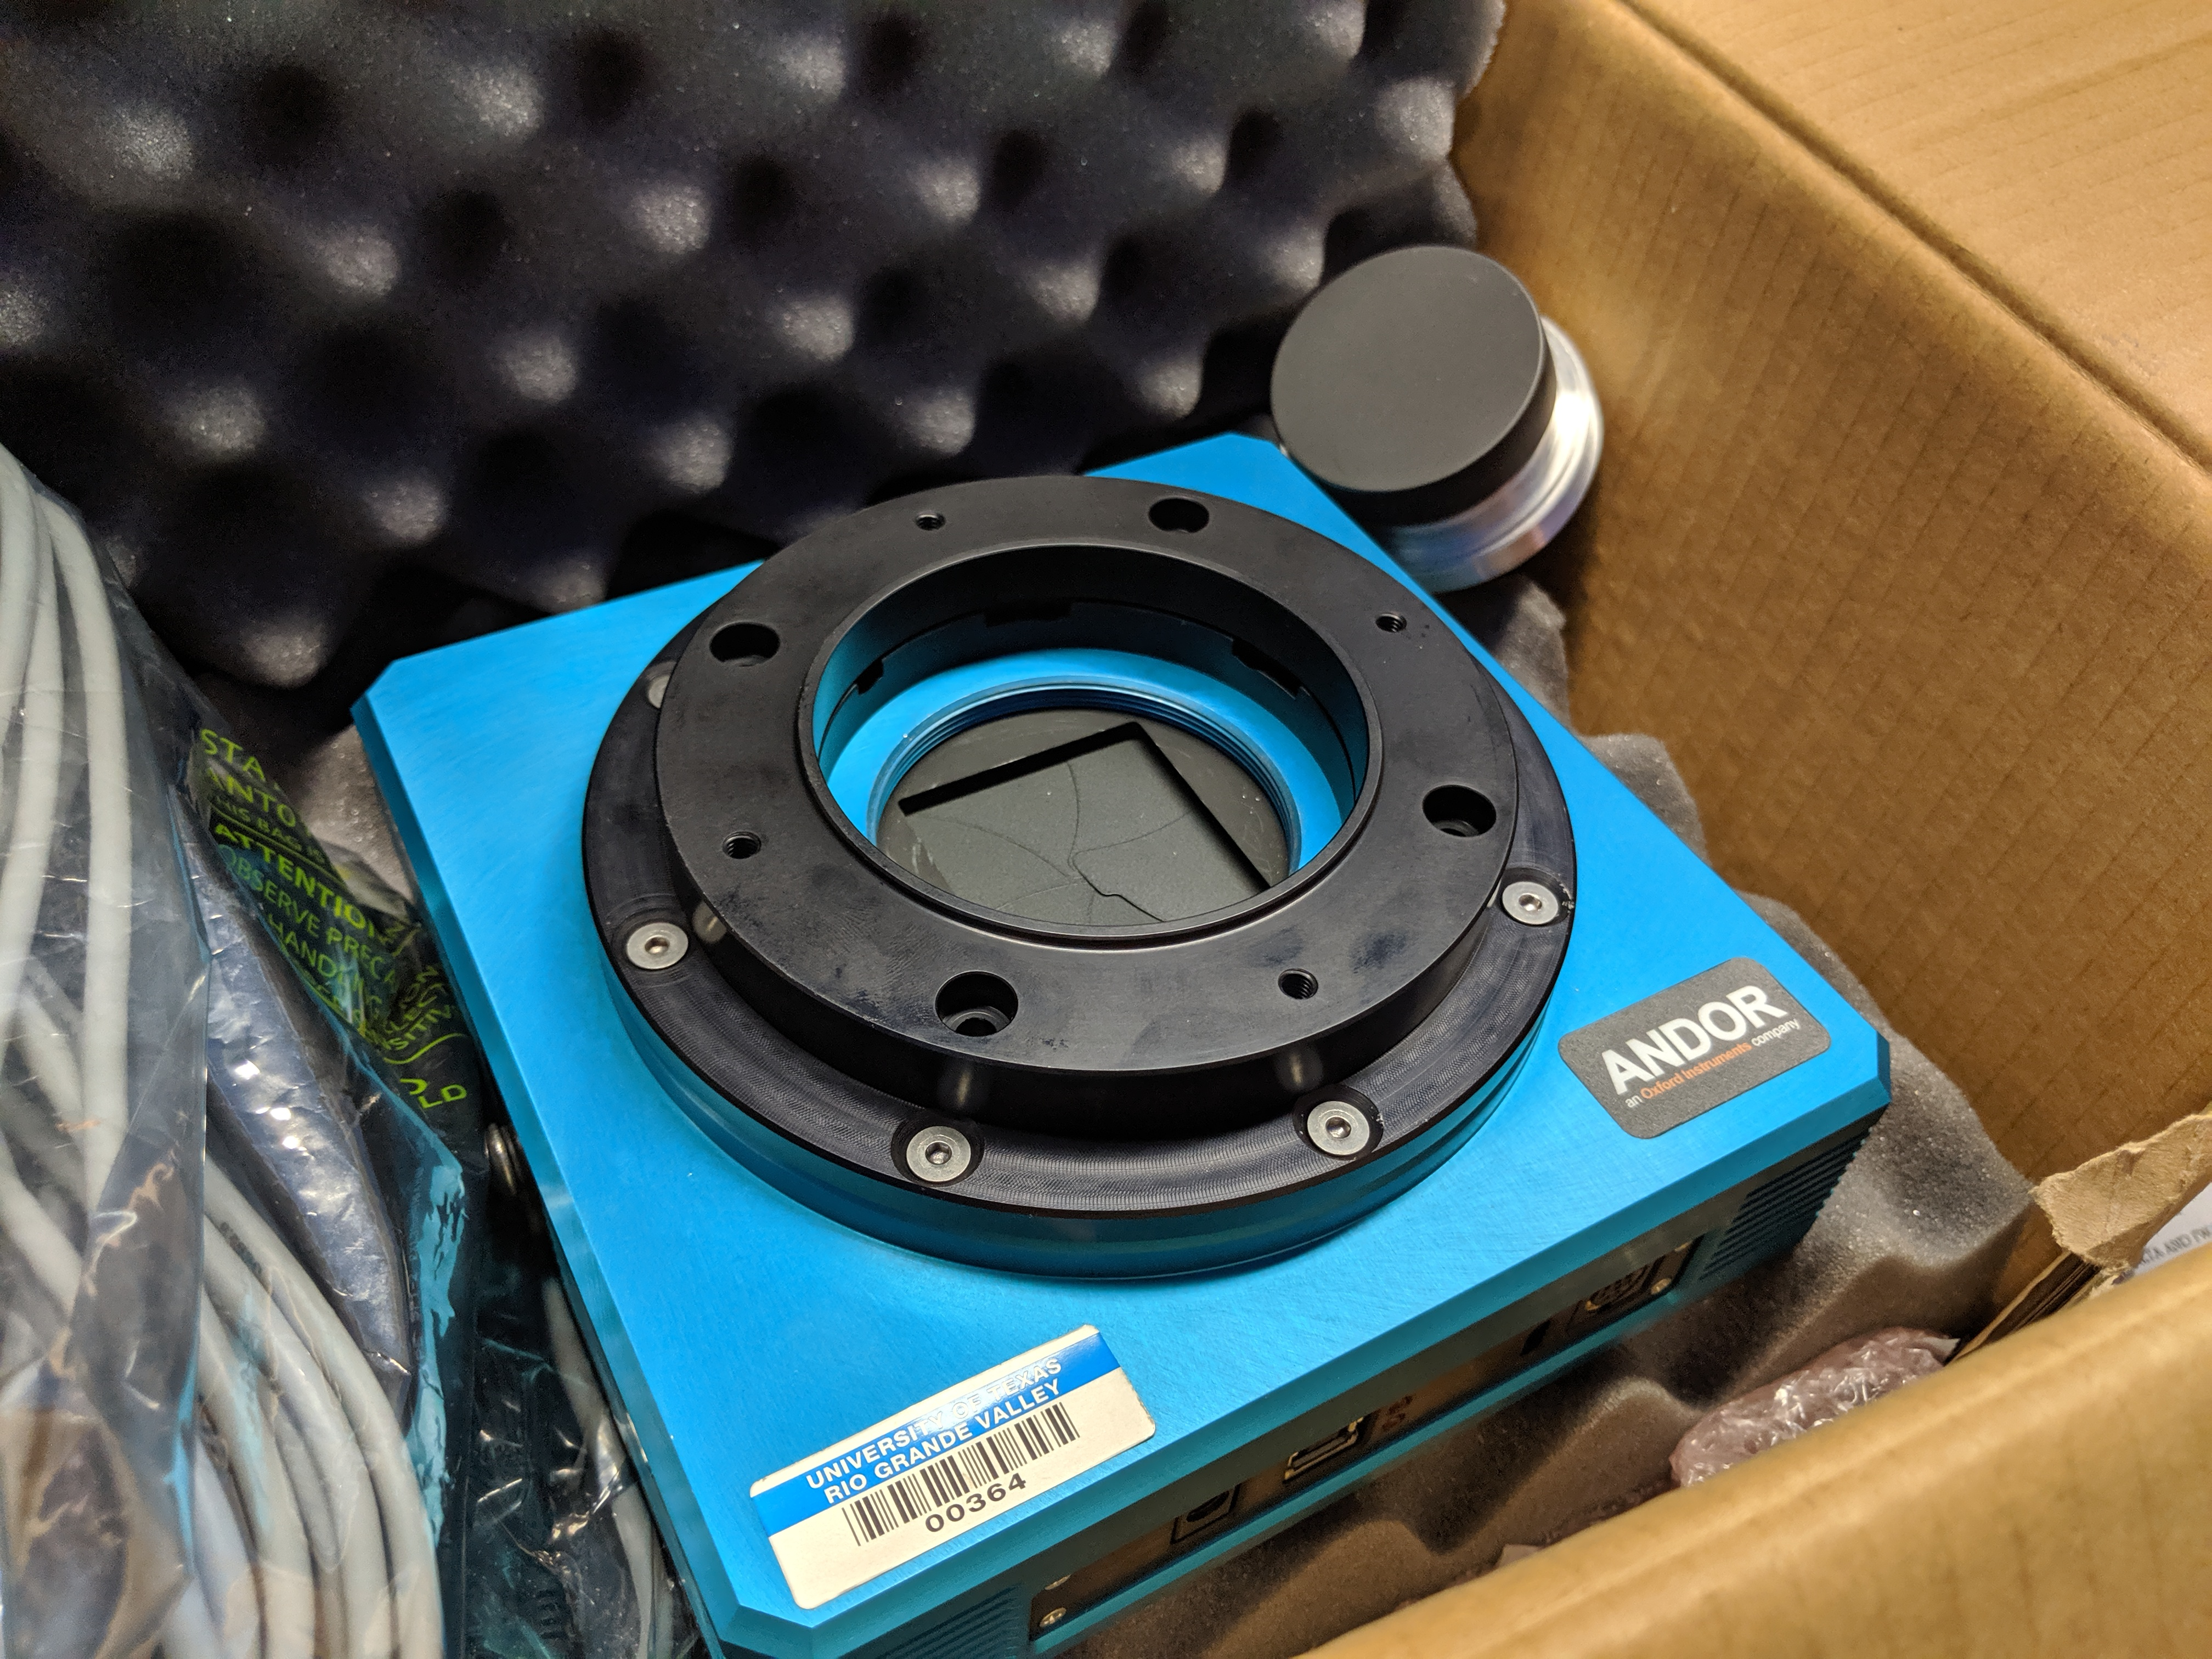
\includegraphics[width=0.5\columnwidth]{figures/apogee.jpg}
    \caption{Apogee Alta F16M being prepared for mounting onto CDK17}
\label{fig:apogee}
\end{figure}

The following specifications are given by the manufacturer ANDOR~\cite{apogee}.
\subsubsection{Specifications}
\begin{description}
    \item[CCD] Kodak KAF-16801
    \item[Pixel Size] $9 \times \SI{9}{\micro\meter}$
    \item[Pixel Array] $4096 \times 4096$ pixels
    \item[CCD Size] $36.8 \times \SI{36.8}{\milli\meter}$
    \item[Read noise] $\SI{7.4}{\elementarycharge}$
    \item[Weight] 4.2 pounds
\end{description}
Linearity tests of the Apogee Alta have been performed and documented by Camuccio~\cite{richard_2019a} to measure gain and read noise.
A plot of the mean pixel value vs the exposure time is show in figure~\ref{fig:linearityapogee}.
\begin{figure}[h]
    \centering
    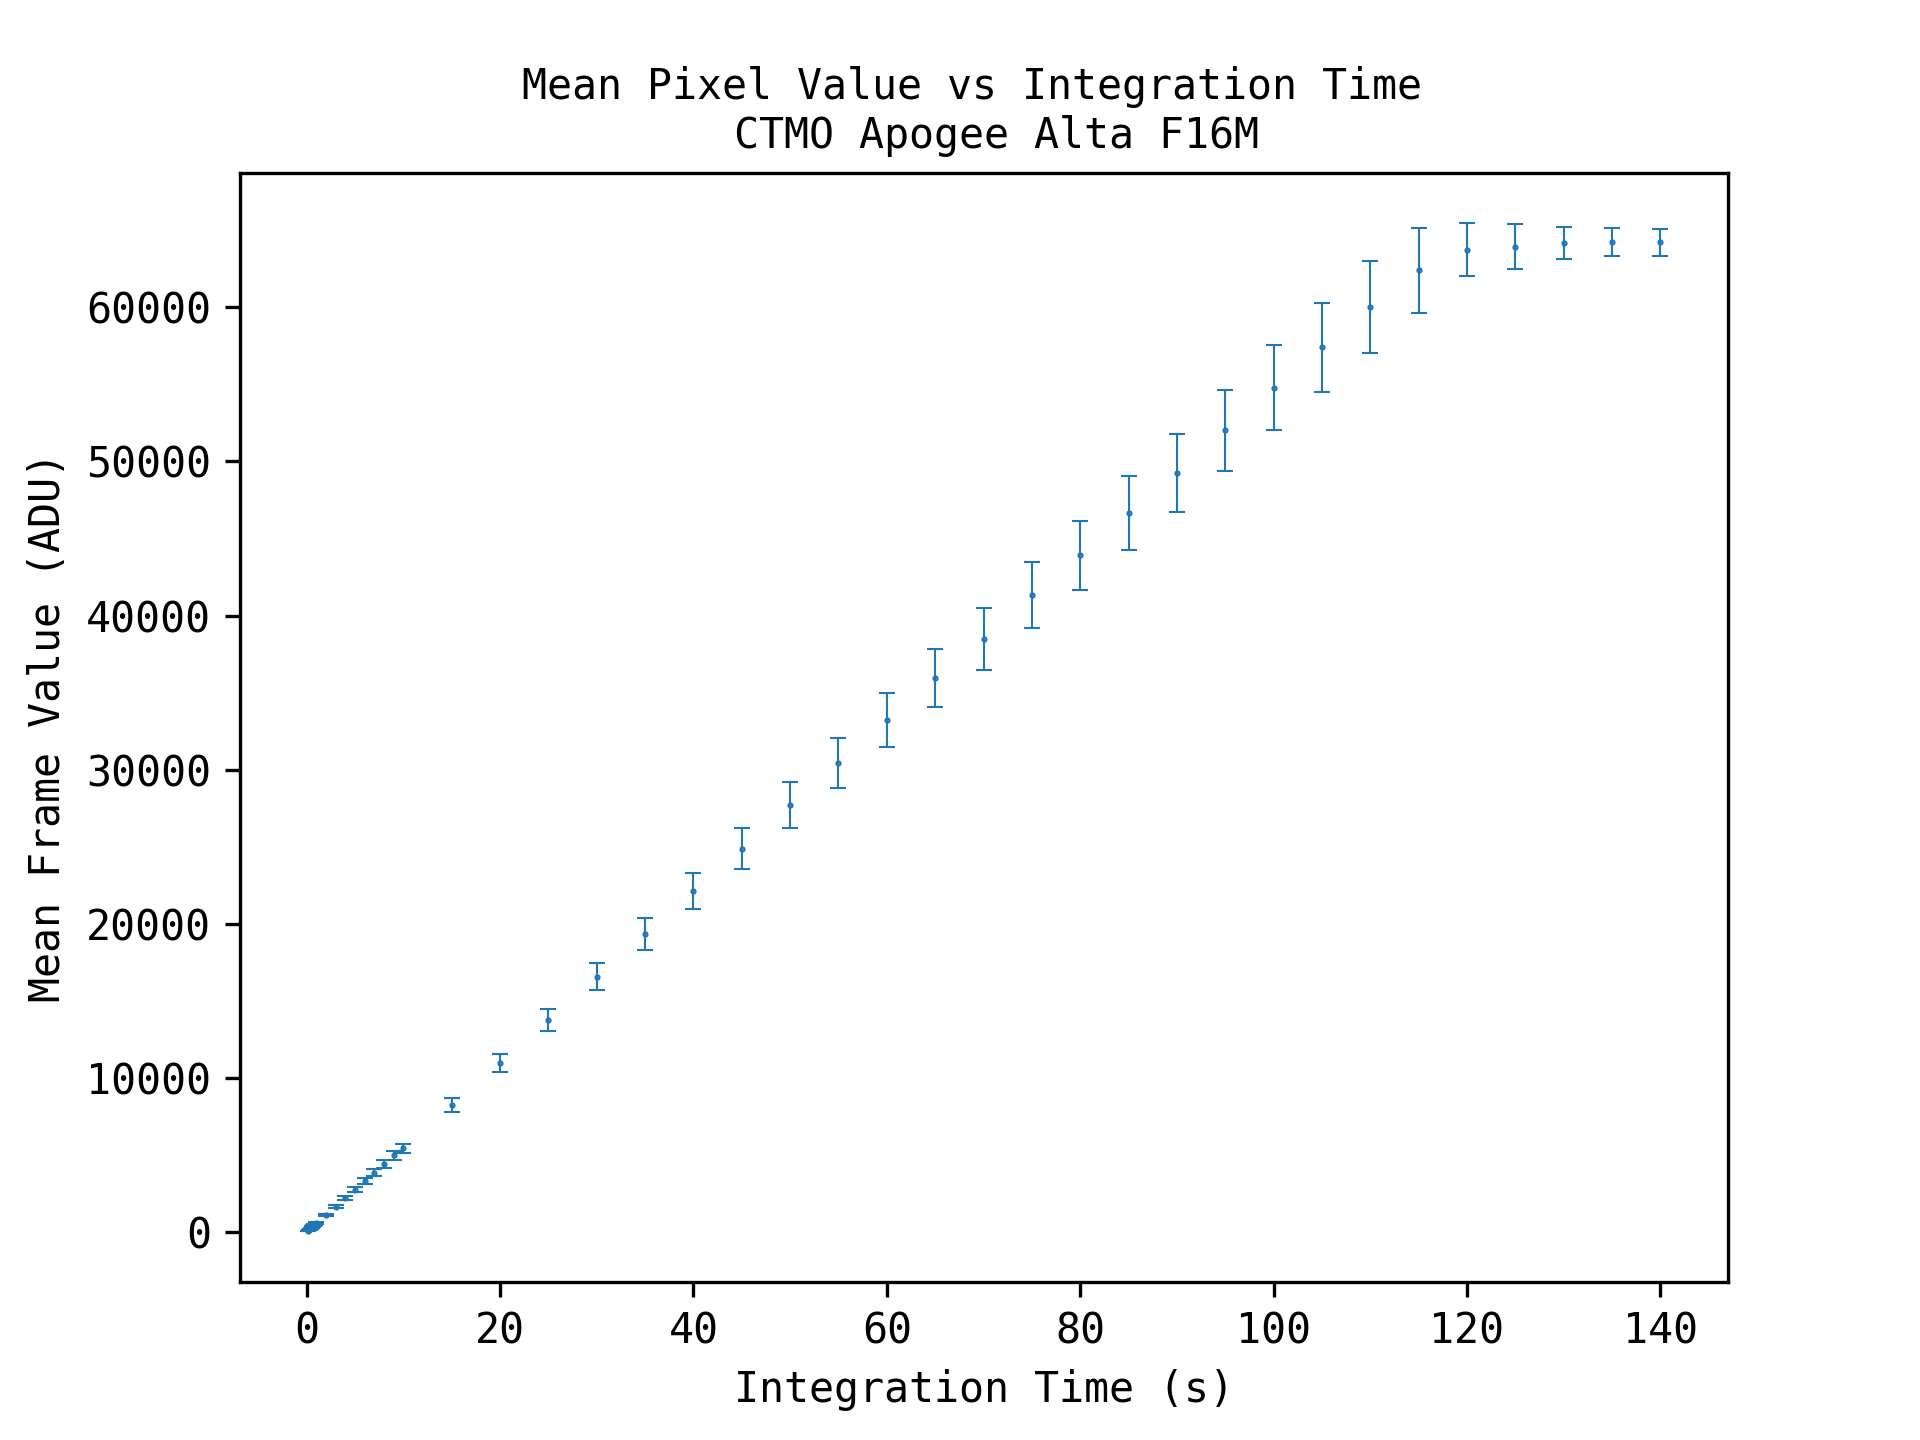
\includegraphics[width=\columnwidth]{figures/apogee_linearity.png}
    \caption{Linearity test of Apogee Alta performed by Richard Camuccio~\protect\cite{richard_2019a}}
\label{fig:linearityapogee}
\end{figure}


\subsubsection{16-inch Meade}
Using equations~\ref{eq:pixelscale} and~\ref{eq:fov} to find pixel scale and FOV, respectively, we find, 
\begin{description}
    \item[Pixel scale] \SI{0.457}{\arcsecond\per\text{pixel}}
    \item[FOV] $\SI{31.18}{\arcminute} \times \SI{31.18}{\arcminute}$
\end{description}

\subsubsection{CDK17}
Using equations~\ref{eq:pixelscale} and~\ref{eq:fov} to find pixel scale and FOV, respectively, we find, 
\begin{description}
    \item[Pixel scale] \SI{0.63}{\arcsecond\per\text{pixel}}
    \item[FOV] $\SI{43.12}{\arcminute} \times \SI{43.12}{\arcminute}$
\end{description}

\section{Software}
CTMO has a Github page where software is being developed at \url{https://github.com/CTMObservatory}
Software used was Maxim DL~\cite{maxim}, Cartes du Ciel-The Sky~\cite{cdc}, ASCOM Platform (POTH)~\cite{ascom},
PWI3/PWI4\cite{planewave}, and INDI Library~\cite{indi}.

\subsection{Dome}
The author is leading the design and development of the custom software for the arduino.
A custom ASCOM driver was written by Latifah Maasarani~\cite{maasarani_2017} to interface 
with an arduino. 
Arduino code is being written by Martin Beroiz.

\begin{figure}[h]
    \centering
    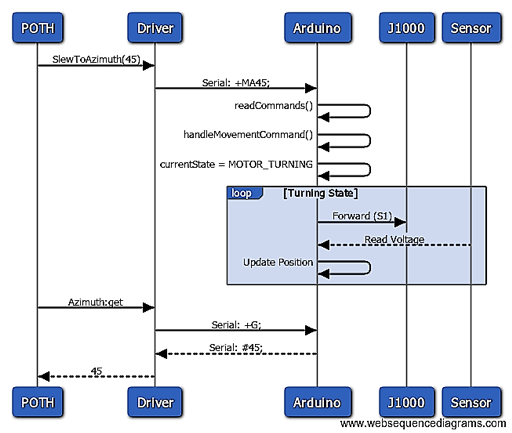
\includegraphics[width=\columnwidth]{figures/driver.png}
    \caption{Sequence diagram for a movement command from POTH platform as implemented by Maasarani~\protect\cite{maasarani_2017}}
\label{fig:driver}
\end{figure}

\subsection{Telescope}
\begin{description}
    \item[Maxim DL] Used for 16-in Meade with ASCOM to attached WCS and pointing information to data
    \item[Cartes du Ciel] Used for 16-in Meade with LX200 Driver and ASCOM Platform separately 
    \item[PWI3] Used for focusing and controlling fans on CDK17
    \item[PWI4] Used for pointing CDK17
\end{description}

\subsection{Camera}
\begin{description}
    \item[Maxim DL] Used for controlling Camera coolers, Filter wheels, and plate solving.
\end{description}

\subsection{Observatory Control System}
This section explains the different observatory control systems implemented during use.
Observatory controls unify the different hardware, drivers, and software. 
Use of systems like this allow for ease of use and proper storage of of data including World Coordinate System (WCS) attachment to 
the file headers of images.

\subsubsection{POTH}
POTH stands for Plain Old Telescope Handset. It uses a framework called ASCOM\@.
ASCOM uses Windows COM protocols to communicate with the drivers required to operate equipment with the computer.
POTH acts as a hub for all communications between drivers, devices, and programs to allow instruments to be used simultaneously 
on different programs.
\begin{figure}[h]
    \centering
    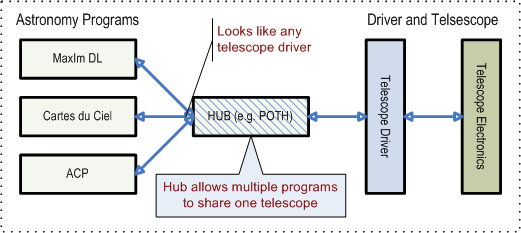
\includegraphics[width=\columnwidth]{figures/poth.png}
    \caption{POTH block diagram of typical usage from ASCOM website~\protect\cite{ascom}}
\label{fig:poth}
\end{figure}

\subsubsection{INDI}
INDI stands for Instrument Neutral Distributed Interface.
According to the INDI website\footnote{\url{http://www.indilib.org}}, INDI Library is an open source architecture for control and automation of astronomical devices.

\subsection{POTH vs INDI}
Both frameworks offer the same service, but were specific to operating system until more recently.
INDI is working on a windows port, but it is in very early stages. 
There is a group called Cloudmakers\footnote{\url{http://www.cloudmakers.eu/windi/}} that made an INDI wrapper and server for Windows.
The INDI wrapper bridges INDI commands with ASCOM protocols.

ASCOM now has an option for Unix based systems that works off of RESTful API and TCP/IP
commands to communicate with drivers and clients called ASCOM Alpaca.
According to the Alpaca developer's webpage\footnote{\url{https://ascom-standards.org/Developer/Alpaca.htm}},
Alpaca is 100 percent independent of Windows. Nowhere in the Alpaca ecosystem is Windows (or COM) needed.
